%%%%%%%%%%%%%%%%%%%%%%%%%%%%%%%%%%%%%%%%%%%%%%%%%%%%%%%%%%%%%%%%%%%%%%%%%%%%%%%%%%%%%%%%%%%%%%%%%%%%%%%%%%%%%%%%%%%%%%%%

%%%%%%%%%%%%%%%%%%%%%%%%%%%%%%%%%%%%%%%%%%%%%
\chapter[Characterizing and predicting network robustness]{Characterizing and predicting network robustness \footnote[3]{A journal article entitled ``Characterizing and Predicting the Robustness of Power-law Networks'' is currently undergoing a second round of review with \emph{Reliability Engineering \& System Safety} \cite{LaRocca2014a}; this paper is based on the random failures portion of the work in this chapter.  A second paper, based on the targeted attacks portion of this work, is in preparation and will be submitted to \emph{Risk Analysis}.}}
\label{ch2}
%%%%%%%%%%%%%%%%%%%%%%%%%%%%%%%%%%%%%%%%%%%%%

%%%%%%%%%%%%%%%%%%%%%%%%%%%%%%%%%%%%%%%%%%%%%%%%%%%%%%%%%%%%%%%%%%%%%%%%%%%%%%%%%%%%%%%%%%

%%%%%%%%%%%%%%%%%%%%%%%%%%%%%%%%%%%%%%%%%%%%%
\section{Introduction}
\label{sec:ch2:intro}
%%%%%%%%%%%%%%%%%%%%%%%%%%%%%%%%%%%%%%%%%%%%%

As discussed in Chapter \ref{ch1}, properly functioning networks are critical to modern life and economies. Communicationsv networks, power systems, and transportation networks form the basis on which economic growth and security is built. The natural environment too is built largely of networks, from cellular metabolic pathways to large-scale ecological networks. In all cases, these networks are subject to failures of critical nodes and links. Communication hubs may be attacked or experience technical failures, bridge failures may lead to large-scale disruption in a transportation network as in the I-35 bridge failure \cite{Sander2007}, power networks may fail due to loss of lines and generation nodes, and ecological networks are subject to severe disruption as species become less common in the network. Being able to quickly and efficiently estimate the ability of a given network to withstand node failures, that is, its robustness, is central to being able to manage critical networks and increase their robustness. At the same time, being able to quickly and efficiently estimate robustness enables more efficient attacks on networks, such as terrorist networks, that we wish to degrade. However, there does not yet exist a method for estimating the robustness of networks quickly and accurately based on the topological characteristics of the network, and the existing understanding of the influence of topological characteristics on network robustness is limited. In this chapter I focus on scale-free networks and develop such a model.

Scale-free networks exhibit a power-law nodal degree distribution where the probability that a given node is connected to $k$ other nodes is described by $P(k) \sim k^{-\gamma}$ \cite{Barabasi1999}. Empirical evidence indicates that nodal degree in many real networks is limited by the physical costs of adding links to a node. Such networks can be described by adding an exponential cutoff to the power-law distribution $P(k) \sim k^{-\gamma}e^{-(k/\kappa)}$, where $\kappa$ is the cutoff above which it becomes physically very costly to add links to a node \cite{Amaral2000,Jeong2000,Newman2001,Clauset2009}. Scale-free networks have been demonstrated to be tolerant to random failures \cite{Albert2000}. However, the combined influence of individual measures of network topology on failure tolerance has not been studied. Without an understanding of the relationship between topology and robustness to node failures, we are limited in our ability to design failure-tolerant networks across many different domains and in our ability to efficiently degrade networks that we wish to attack. In this chapter, I present a systematic study of the effects of topological characteristics on power-law network fault tolerance, and I develop a topology-based statistical approach for estimating the ability of a network to tolerate node failures.

My work helps to address the gap in current network robustness modeling in two ways. First, I develop a statistical model for quickly estimating the robustness of a network after node failure events for networks containing up to 1,000 nodes. This model estimates robustness for up to 75\% of the original nodes failing, making it useful not only for small failure events but also large-scale failure events induced by common-cause failures such as natural disasters in which large portions of networks fail \cite{Han2009a, Han2009b, Guikema2010, Nateghi2011}. Second, I use my statistical model to gain insight into the topological characteristics of networks that influence their robustness. This, together with rapid estimation of robustness, provides a strong basis on which robustness can be included in network design optimization.

%%%%%%%%%%%%%%%%%%%%%%%%%%%%%%%%%%%%%%%%%%%%%%%%%%%%%%%%%%%%%%%%%%%%%%%%%%%%%%%%%%%%%%%%%%

%%%%%%%%%%%%%%%%%%%%%%%%%%%%%%%%%%%%%%%%%%%%%
\section{Methods}
\label{sec:ch2:methods}
%%%%%%%%%%%%%%%%%%%%%%%%%%%%%%%%%%%%%%%%%%%%%

%%%%%%%%%%%%%%%%%%%%%%%%%%%%%%%%%%%%%%%%%%%%%%%%%%%%%%%%%%%%%%%%%%%%%%%%%%%

%%%%%%%%%%%%%%%%%%%%%%%%%%%%%%%%%%%%%%%%%%%%%
\subsection{Simulation}
\label{sec:ch2:methods:simulation}
%%%%%%%%%%%%%%%%%%%%%%%%%%%%%%%%%%%%%%%%%%%%%

Prior work on network robustness focuses on relatively small numbers of networks due to the limited number of real networks for which data is available \cite{Holme2002, Jeong2001, Albert2004, Crucitti2004a, Estrada2006, Montoya2006, Liu2011}. However, this significantly limits the statistical strength of the insights that can be drawn from the analysis. To overcome this limitation, I begin by randomly generating 2,000 networks with degree distributions following a power-law with exponential cutoff and distribution parameters representative of scale-free networks in a variety of domains \cite{Albert2002}. My algorithm is a variation on preferential attachment and is provided in Appendix \ref{appA}.

This algorithm is not guaranteed to produce a connected network, so after generating a network I check to see if it is fully connected using a breadth-first search. If the network is not connected, I discard it and try again. For most degree distributions and parameters I am able to generate a connected network in a very small number of attempts (\textbf{$<5$}).  I use five pairs of distribution parameters, based on the network data presented in \cite{Albert2002} (Tables \ref{tab:ch1:degreedist1} and \ref{tab:ch2:powerlawparams}).  I generate 400 random networks for each parameter combination: 20 networks for each of 20 sizes (Table \ref{tab:ch2:networkSize}). The network sizes between 100 and 1000 are generated from a uniform random distribution.

%--------------------------------------------
% TABLE -------------------------------------

\begin{table}
\centering

\begin{tabular}{rr}
\toprule
$\mathbf{\gamma}$ & $\mathbf{\kappa}$\\
\midrule
1.1 & 40\\
2.0 & 900\\
2.1 & 400\\
2.4 & 2,000\\
1.7 & 200\\
\bottomrule

\end{tabular}

\caption{\label{tab:ch2:powerlawparams}Power-law with exponential cutoff degree distribution parameters used for generating networks.}
\end{table}

%--------------------------------------------

%--------------------------------------------
% TABLE -------------------------------------

\begin{table}
\centering

\begin{tabular}{ccc}
\toprule
\textbf{Number of} & \textbf{Number of} & \textbf{Number of}\\
\textbf{nodes} & \textbf{degree distributions} & \textbf{networks}\\
\midrule
100 & 5 & 20\\
126 & 5 & 20\\
177 & 5 & 20\\
205 & 5 & 20\\
299 & 5 & 20\\
313 & 5 & 20\\
336 & 5 & 20\\
367 & 5 & 20\\
387 & 5 & 20\\
482 & 5 & 20\\
513 & 5 & 20\\
540 & 5 & 20\\
557 & 5 & 20\\
592 & 5 & 20\\
621 & 5 & 20\\
758 & 5 & 20\\
821 & 5 & 20\\
936 & 5 & 20\\
967 & 5 & 20\\
1000 & 5 & 20\\

\bottomrule

\end{tabular}

\caption[]{\label{tab:ch2:networkSize}Summary of number and sizes of networks generated.}
\end{table}

%--------------------------------------------

After generating these networks, I calculate the mean, standard deviation, minimum, and maximum values of four topological characteristics for each network individually.  Table \ref{tab:ch2:networkStats} presents the mean, standard deviation, minimum, and maximum of each of these network-level summary statistics: nodal degree ($\mu = 5.13$), clustering coefficient \cite{Watts1998} ($\mu = 0.289$), betweenness centrality \cite{Freeman1977} ($\mu = 746$) and path length ($\mu = 2.47$).  Figures \ref{fig:ch2:degreeStats}-\ref{fig:ch2:pathLengthStats} show the histograms of the mean, standard deviation, minimum, and maximum topological characteristics for all networks generated. The ranges for my network characteristics are similar to ranges for real networks such as the Internet, movie actors, scientific paper co-authorship, metabolic reactions, food webs, and word synonyms as presented in \cite{Albert2002}. The mean degree of the networks ranges from 2.3 to 11.2 and the mean degree of networks in \cite{Albert2002} ranges from 2.39 to 173, though only a few non-physical networks such as word associations and social networks reported in \cite{Albert2002} have a mean nodal degree greater than 18. The mean clustering coefficient of my networks ranges from 0.067 to 0.61 and the mean clustering coefficient of networks in \cite{Albert2002} ranges from 0.066 to 0.79. The mean path length of my networks ranges from 2.0 to 3.3 and the mean path length of networks in \cite{Albert2002} ranges from 2.4 to 18.7, though the path lengths for power-law networks reported by \cite{Albert2002} are close to those of my network with the exception of several social networks.

%--------------------------------------------
% FIGURE ------------------------------------

\begin{figure}[!htp]
\centering
\centerline{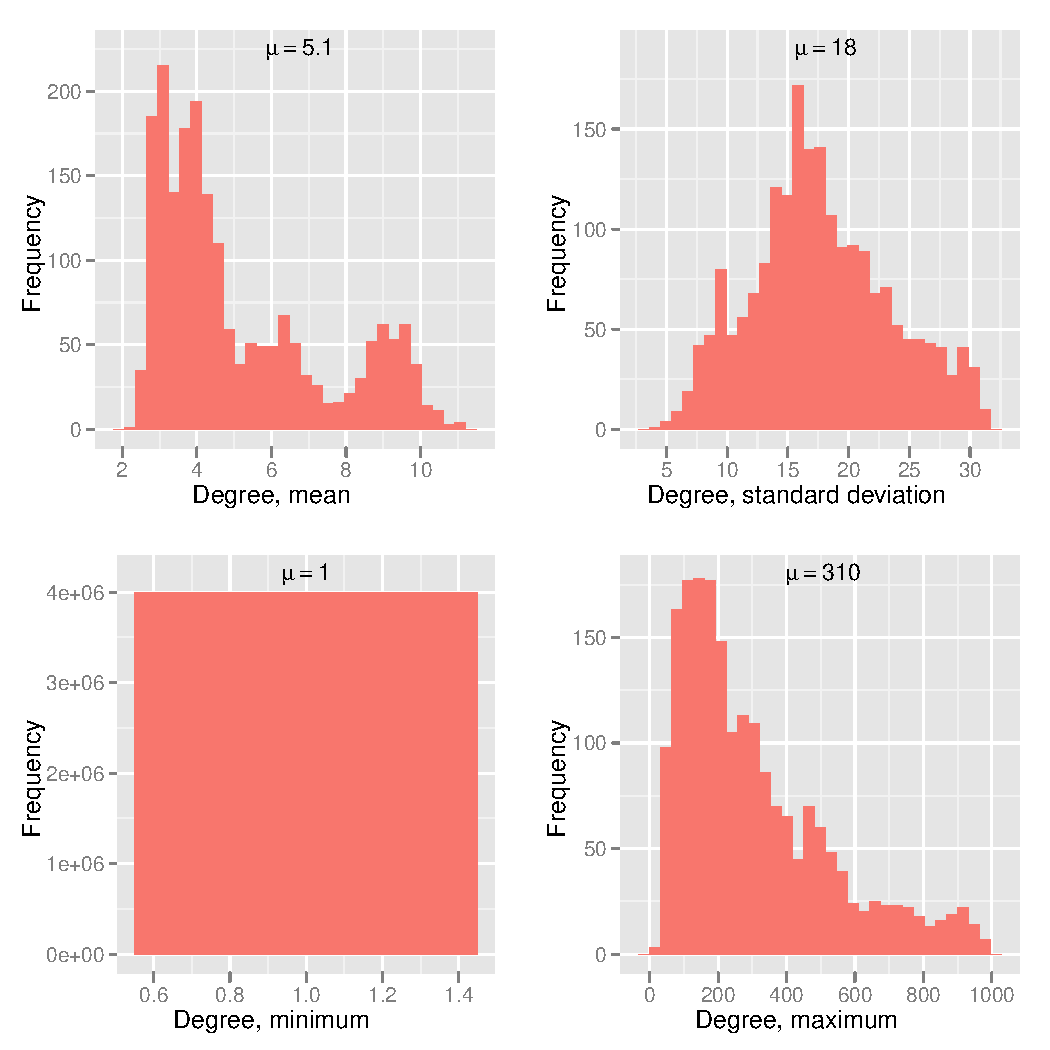
\includegraphics[width=\textwidth]{degreeStatsPlot.pdf}}
\caption{\label{fig:ch2:degreeStats}Distribution of network topologies: degree.}
\end{figure}

%--------------------------------------------

%--------------------------------------------
% FIGURE ------------------------------------

\begin{figure}[!htp]
\centering
\centerline{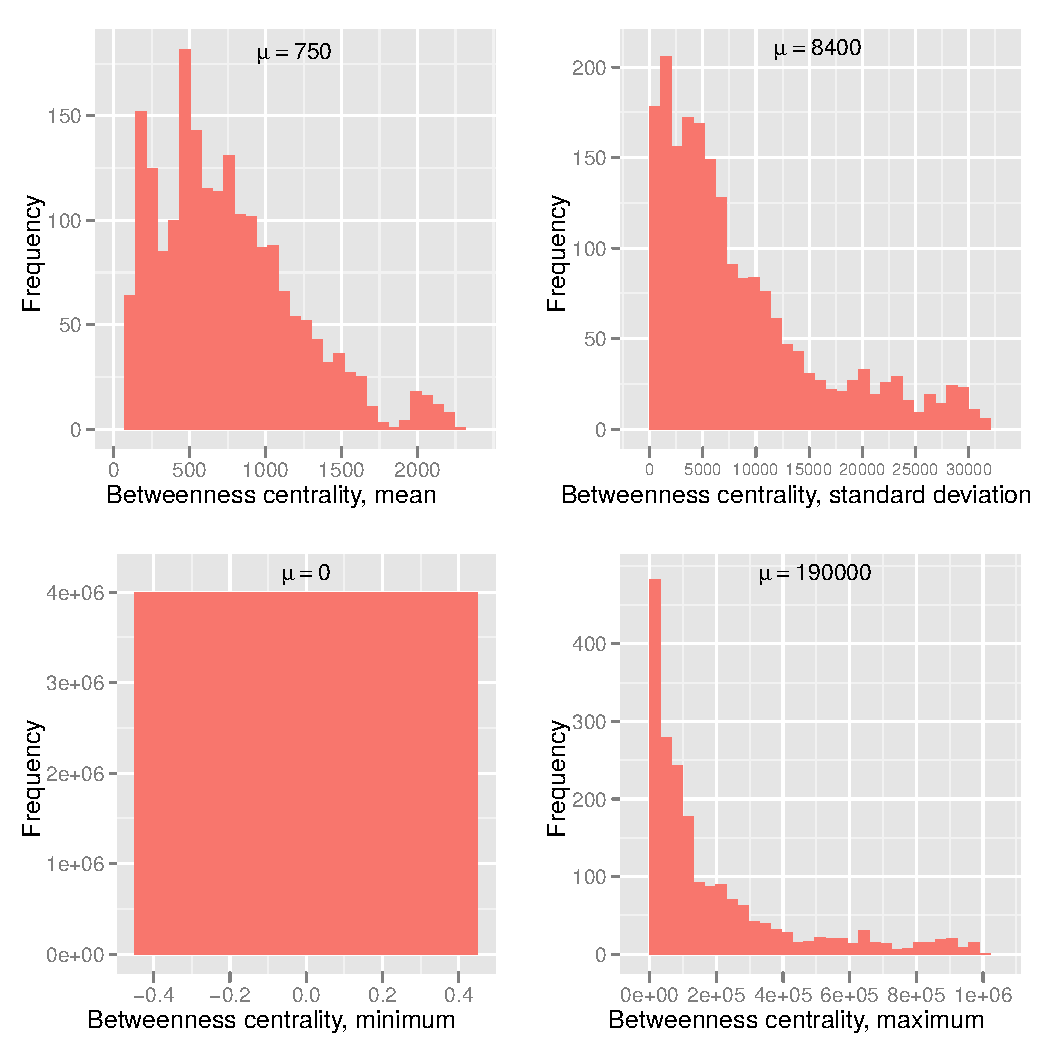
\includegraphics[width=\textwidth]{betweennessStatsPlotV2.pdf}}
\caption{\label{fig:ch2:betweennessStats}Distribution of network topologies: betweenness centrality.}
\end{figure}

%--------------------------------------------

%--------------------------------------------
% FIGURE ------------------------------------

\begin{figure}[!htp]
\centering
\centerline{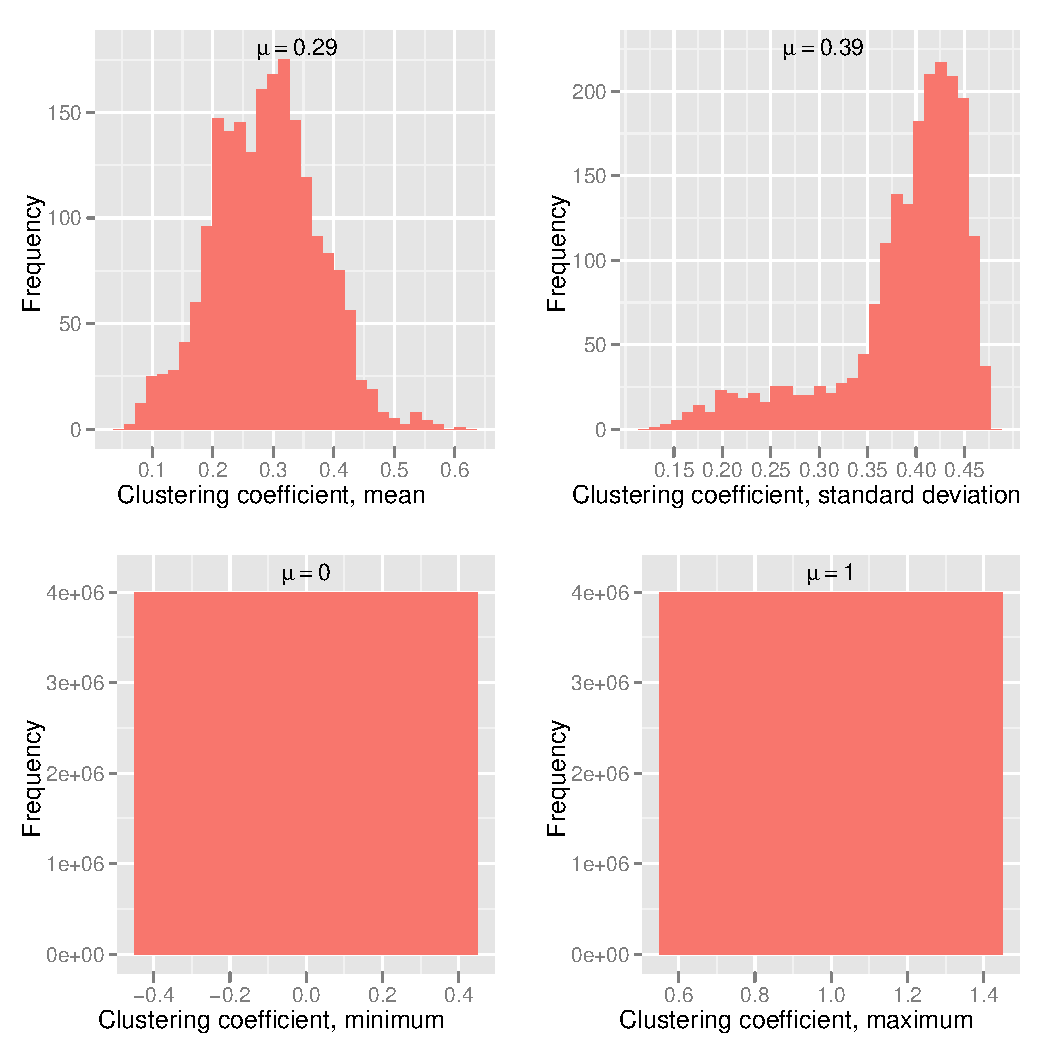
\includegraphics[width=\textwidth]{clusteringStatsPlot.pdf}}
\caption{\label{fig:ch2:clusteringStats}Distribution of network topologies: clustering coefficient.}
\end{figure}

%--------------------------------------------

%--------------------------------------------
% FIGURE ------------------------------------

\begin{figure}[!htp]
\centering
\centerline{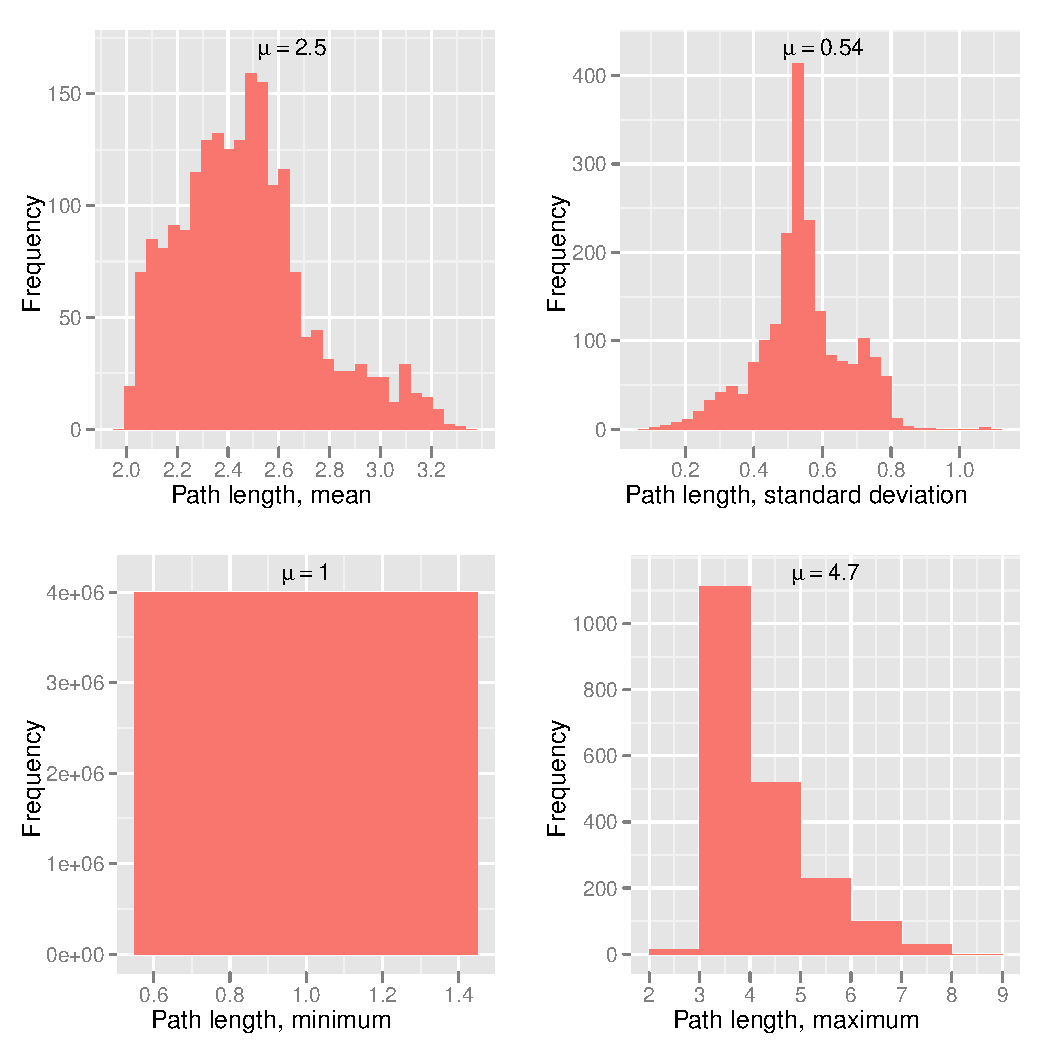
\includegraphics[width=\textwidth]{pathLengthStatsPlot.pdf}}
\caption{\label{fig:ch2:pathLengthStats}Distribution of network topologies: path length.}
\end{figure}

%--------------------------------------------

%--------------------------------------------
% TABLE -------------------------------------

\begin{table}[!htp]
\scriptsize
\centering

\begin{tabular}{lccccc}
\toprule
\textbf{Parameter} & \textbf{Within-network} & \textbf{Mean} & \textbf{Standard} & \textbf{Minimum} & \textbf{Maximum}\\
& \textbf{measure} & & \textbf{deviation} & & \\
\midrule

Network size ($n$) & & 505 & 272 & 100 & 1000\\
\multirow{4}{*}{Degree ($k$)} & \textbf{Mean} & 5.1 & 2.2 & 2.3 & 11.2\\
& Minimum & 1.0 & 0.0 & 1.0 & 1.0\\
& Maximum & 307 & 220 & 24 & 989\\
& Standard deviation & 17.7 & 5.7 & 4.5 & 31.7\\
\multirow{4}{*}{Betweenness centrality ($Cb$)} & \textbf{Mean} & 746 & 452 & 105 & 2,278\\
& Minimum & 0.0 & 0.0 & 0.0 & 0.0\\
& Maximum & 192,468 & 229,924 & 1,808 & 992,170\\
& Standard deviation & 8,433 & 7,495 & 316 & 31,375\\
\multirow{4}{*}{Clustering coefficient ($C$)} & \textbf{Mean} & 0.29 & 0.09 & 0.07 & 0.61\\
& Minimum & 0.0 & 0.0 & 0.0 & 0.0\\
& Maximum & 1.0 & 0.0 & 1.0 & 1.0\\
& \textbf{Standard deviation} & 0.39 & 0.07 & 0.13 & 0.48\\
\multirow{4}{*}{Path length ($\ell$)} & Mean & 2.5 & 0.3 & 2.0 & 3.3\\
& Minimum & 1.0 & 0.0 & 1.0 & 1.0\\
& \textbf{Maximum} & 4.7 & 0.96 & 3.0 & 8.0\\
& \textbf{Standard deviation} & 0.5 & 0.1 & 0.1 & 1.1\\


\bottomrule

\end{tabular}

\caption[Summary of topological characteristics of generated networks.]{\label{tab:ch2:networkStats}Summary of the topological characteristics of generated networks. Bolded characteristics indicate those included in final regression models.}
\end{table}

%--------------------------------------------

I then repeatedly and independently simulate 100 random node failure scenarios for each network, with equal failure probability for each node, varying the number of nodes failed from $0.10 N_0$ up to $0.75 N_0$, where $N_0$ is the number of nodes in the initial, unperturbed network. These node failure events result in disconnection of one or more nodes from the remainder of the network. My measure of network robustness is:
%
\begin{equation}
S^p = \frac{N^p_f}{N_0},
\end{equation} 
%
where $N^p_f$ is the total number of nodes in the largest connected component after $p$ percent of nodes have failed. $S^p$ thus gives us the relative size of the largest connected component, a measure of the degree to which the network maintains topological integrity after node failure events \cite{Albert2000}. I calculate $S$ for each failure scenario in each network at four failure levels: 10, 25, 50, and 75 percent of nodes failed. I also develop four additional targeted node failure scenarios, where nodes fail one at a time until all nodes have failed, with the node of highest importance failing first and the node of least importance failing last.  If two or more nodes are ranked equally, their failure order is selected uniform randomly. Node importance is defined in four ways based on the following node characteristics: 1) initial degree; 2) recalculated degree after each node failure; 3) initial betweenness; and  4) recalculated betweenness after each node failure. Table \ref{tab:ch2:robustnessStats} provides a summary of values of $S$ for each level of node failure for the random and targeted failure scenarios.

%--------------------------------------------
% TABLE -------------------------------------

\begin{table}[!htp]
\centering
\scriptsize
\begin{tabular}{lccccc}
\toprule
\multirow{2}{*}{\textbf{Failure type}} & \multicolumn{4}{c}{$S$ \textbf{after nodes removed}}\\
 & {10\%} & {25\%} & {50\%} & {75\%}\\
\midrule
Random & $0.85\,(0.81,0.88)$ & $0.64\,(0.58, 0.69)$ & $0.33\,(0.27,0.40)$ & $0.11\,(0.070,0.15)$\\
Targeted, initial degree & 0.12 & 0.010 & 0.0037 & 0.0030 \\
Targeted, recalculated degree & 0.12 & 0.0046 & 0.0030 & 0.0030 \\
Targeted, initial betweenness & 0.13 & 0.022 & 0.0034 & 0.0031 \\
Targeted, recalculated betweenness & 0.12 & 0.0066 & 0.0059 & 0.0057 \\

\bottomrule

\end{tabular}

\caption[Summary of relative size of largest connected component after failure simulations.]{\label{tab:ch2:robustnessStats}Summary of mean values of relative size of largest connected component after failure simulations. Values in parentheses for random failures represent the 95\% confidence interval for the 100 failure simulations.}
\end{table}

%--------------------------------------------

%%%%%%%%%%%%%%%%%%%%%%%%%%%%%%%%%%%%%%%%%%%%%%%%%%%%%%%%%%%%%%%%%%%%%%%%%%%

%%%%%%%%%%%%%%%%%%%%%%%%%%%%%%%%%%%%%%%%%%%%%
\subsection{Regression modeling}
\label{sec:ch2:methods:regression}
%%%%%%%%%%%%%%%%%%%%%%%%%%%%%%%%%%%%%%%%%%%%%

Classical linear regression models can be described as follows.  Let $\mathbf{y}$ be a vector of $n$ observations, $\mathbf{y} = \{y_1, \ldots , y_n\}^T$.  And, let $\mathbf{X}$ be a matrix of explanatory variables of size $n \times p$, where $p$ is the number of covariates.  We then define a set of parameters, $\beta = \{\beta_1, \ldots , \beta_p\}^T$ used to relate $\mathbf{X}$ to $\mathbf{y}$.  Typically, the vector $\beta$ is found by minimizing the square of the residuals between $\mathbf{y}$ and $\mathbf{X\beta}$, that is:
%
\begin{equation}
\mathrm{minimize}_\beta (\mathbf{y}-\mathbf{X}\bm{\beta})(\mathbf{y}-\mathbf{X}\bm{\beta})^T.
\end{equation}
%
In this classical linear model, we assume that each of our observations, $y_i$ follows from a Normally-distributed random variable $Y_i$ with mean $\mu_i$ and constant variance, $\sigma^2$.  Thus, we have:
%
\begin{equation}
E(\mathbf{Y}) = \bm{\mu}.
\end{equation}
%
This is what is known as the \emph{random component} of this model.  The \emph{systematic component} of this model relates $\bm{\mu}$ to $\mathbf{X}$ and $\bm{\beta}$:
%
\begin{equation}
\mu_i = \sum\limits_1^p{x_{ij}}\beta_j; \;\;    i = 1,\ldots, n,
\end{equation}
%
where $i$ is the observation and $j$ is the covariate. We can also write this in matrix form as:
%
\begin{equation}
\bm{\mu} = \mathbf{X}\bm{\beta}.
\end{equation}

As previously described, a critical component of classical linear models is the assumption that the components of $\mathbf{Y}$ (\emph{i.e.}, our observations) are independent Normal variables with constant variance $\sigma^2$.  However, real data often does not conform to this assumption.  In 1972, Nelder and Wedderburn \cite{Nelder1972} proposed a method for using linear regression with observations distributed according to other distributions in the exponential family; the models obtained from their method are known as \emph{generalized linear models}.

Generalized linear models (GLMs) contain both a \emph{random component} and a \emph{systematic component} as described above.  However, with a GLM, the distribution used in the random component can be any distribution belonging to the exponential family, rather than being assumed to be Normal.  Additionally, GLMs contain a third model component, the \emph{link function}, which relates the random and systematic components as follows.  Suppose we have a random component, $E(\mathbf{Y}) = \bm{\mu}$, and a systematic component, $\bm{\eta} = \mathbf{X}\bm{\beta}$.  Then our link function is defined as $\eta_i =f(\mu_i)$, where $f(\cdot)$ is any monotonic differentiable function.  For classical linear regression models, the link function is the identity function; that is, $\bm{\eta} = \bm{\mu}$.

Because it is a ratio of largest connected component after failures to initial network size, our observed data, $S$, in this analysis is restricted to the interval (0,1). Ferrari and Cribari-Neto \cite{Ferrari2004a} developed a regression model for use with such Beta-distributed response data.\footnote[4]{The Beta regression model proposed by Ferrari and Cribari-Neto offers an improvement on logistic regression models in that it naturally accomodates for heteroskedasticity and assymetries in the rate or proportion response variable \cite{Cribari2010}; this is why I have chosen to use it here.} Their model is not technically a generalized linear model (GLM), because the Beta distribution does not belong to the exponential family. However, their method follows the approach for GLMs first described by Nelder and Wedderburn \cite{Nelder1972} and relies on a reparameterization of the Beta density function, as follows:
%
\begin{equation}
f(y;\mu,\phi) = \frac{\Gamma(\phi)}{\Gamma(\mu\phi)\Gamma((1-\mu)\phi)}y^{\mu\phi - 1}(1-y)^{(1-\mu)\phi - 1}, 0<y<1
\end{equation}
%
The mean and variance using this parameterization can be described as follows:
%
\begin{equation}
\text{E}(y) = \mu
\end{equation}
%
and
%
\begin{equation}
\text{var}(y) = \frac{\mu(1-\mu)}{1+\phi}.
\end{equation}
%
In this model, the components of the response vector, $\mathbf{Y}$, have independent Beta distributions with $E[\mathbf{Y}] = \mathbf{\mu}$. We can write the systematic component as 
%
\begin{equation}
\eta_i = \sum\limits_1^p x_{ij}\beta{j}.
\end{equation}
%
There are a variety of link functions that can be used with the Beta regression model proposed by Ferrari and Cribari-Neto; for my analysis I used the standard logit link function, defined as:
%
\begin{equation}
\mathbf{\eta}=\ln\left(\frac{\mu}{1-\mu}\right).
\end{equation}
%
I use the methodology described above to develop Beta regression models for network robustness. My initial data set includes sixteen explanatory variables: minimum, maximum, mean, and standard deviation values for each of the four topological characteristics of networks previously described. I remove variables with standard deviation equal to zero from my data set because they will have no impact in a regression model. These variables are minimum degree, minimum betweenness, minimum clustering coefficient, maximum clustering coefficient, and minimum path length. To avoid multicollinearity effects from the remaining variables, I remove maximum degree, standard deviation of degree, standard deviation of betweenness, and mean path length from my data set. I then standardize the remaining variables for easier interpretability of model results.

I fit Beta regression models to the reduced data by performing maximum likelihood estimation using the Betareg package \cite{Cribari2010} in [R] \cite{R2012}. Because I calculate $S$ after four levels of node removals (10, 25, 50, and 75 percent), I develop four separate models, with $S$ for a single level of node failures (10, 25, 50, and 75 percent) as the response variable in each model.  After fitting a given initial model, I iteratively remove all covariates from the model that are not statistically significant. That is, for a given model, I remove the explanatory variable with the highest p-value, refit the model, and repeat until all variables are statistically significant at the level of $\alpha = 0.05$.  I repeat this modeling process with the results for all five types of node failures (\emph{i.e.}, random, initial degree-based, recalculated degree-based, initial betweenness-based, and recalculated betweenness-based). Tables \ref{tab:ch2:betaregNR}-\ref{tab:ch2:betaregNBr} contain the parameter estimates and standard errors for each of the twenty total regression models; Table \ref{tab:ch2:pseudorsquared} presents pseudo-R-squared values for each.

%--------------------------------------------
% TABLE -------------------------------------

\begin{table}[!htp]
\scriptsize
\centering

\begin{tabular}{lcccccccc}
\toprule
\multirow{2}{*}{\textbf{Parameter}} & \multicolumn{2}{c}{\textbf{10\%}} & \multicolumn{2}{c}{\textbf{25\%}} & \multicolumn{2}{c}{\textbf{50\%}} & \multicolumn{2}{c}{\textbf{75\%}}\\
 & $\hat{\beta}$ & Std. Err. & $\hat{\beta}$ & Std. Err. & $\hat{\beta}$ & Std. Err. & $\hat{\beta}$ & Std. Err. \\
\midrule

(Intercept) & 1.7 & 0.0019 & 0.56 & 0.0014 & -0.70 & 0.0014 & -2.1 & 0.0019 \\
$k_{mean}$ & 0.051 & 0.0070 & 0.063 & 0.0052 & 0.097 & 0.0048 & 0.16 & 0.0061 \\
$Cb_{mean}$ & -0.0096 & 0.0026 & -0.0041 & 0.0019 & -0.0036 & 0.0018 & -0.008 & 0.0025 \\
$C_{mean}$ & 0.062 & 0.0077 & 0.065 & 0.0057 & 0.071 & 0.0053 & 0.074 & 0.0067 \\
$C_{std dev}$ & -0.067 & 0.0086 & -0.070 & 0.0064 & -0.072 & 0.0060 & -0.062 & 0.0076 \\
$l_{std dev}$ & 0.012 & 0.0028 & 0.014 & 0.0021 & 0.018 & 0.0021 & 0.048 & 0.0035 \\
$l_{max}$ & -- & -- & -- & -- & -- & -- & -0.0074 & 0.0037 \\
$\phi$ & 1100 & 35 & 1100 & 34 & 1200 & 38 & 1600 & 49 \\

\bottomrule

\end{tabular}

\caption[Beta regression model parameters for network robustness to random node failures.]{\label{tab:ch2:betaregNR}Beta regression model parameters for network robustness to random node failures as a function of initial network topology.}
\end{table}

%--------------------------------------------

%--------------------------------------------
% TABLE -------------------------------------

\begin{table}[!htp]
\scriptsize
\centering

\begin{tabular}{lcccccccc}
\toprule
\multirow{2}{*}{\textbf{Parameter}} & \multicolumn{2}{c}{\textbf{10\%}} & \multicolumn{2}{c}{\textbf{25\%}} & \multicolumn{2}{c}{\textbf{50\%}} & \multicolumn{2}{c}{\textbf{75\%}}\\
 & $\hat{\beta}$ & Std. Err. & $\hat{\beta}$ & Std. Err. & $\hat{\beta}$ & Std. Err. & $\hat{\beta}$ & Std. Err. \\
\midrule

(Intercept) & -3.3 & 0.019 & -5.0 & 0.014 & -5.8 & 0.0076 & -6.0 & 0.0060 \\
$k_{mean}$ & 0.69 & 0.025 & 0.12 & 0.026 & -0.053 & 0.018 & -0.21 & 0.017 \\
$Cb_{mean}$ & -0.46 & 0.014 & -0.41 & 0.014 & -0.54 & 0.013 & -0.62 & 0.013 \\
$Cb_{max}$ & NA & NA & NA & NA & -0.13 & 0.015 & -0.073 & 0.012 \\
$C_{mean}$ & 0.58 & 0.028 & 0.23 & 0.030 & 0.19 & 0.019 & 0.17 & 0.017 \\
$C_{std dev}$ & -1.5 & 0.034 & -0.75 & 0.035 & -0.43 & 0.023 & -0.25 & 0.020 \\
$l_{std dev}$ & 0.32 & 0.024 & 0.32 & 0.020 & 0.20 & 0.012 & 0.24 & 0.0090 \\
$l_{max}$ & -0.052 & 0.020 & -0.12 & 0.020 & -0.034 & 0.012 & -0.089 & 0.0099 \\
$\phi$ & 65 & 2.2 & 430 & 14 & 3600 & 110 & 7300 & 230 \\

\bottomrule

\end{tabular}

\caption[Beta regression model parameters for network robustness to initial degree-based attacks.]{\label{tab:ch2:betaregNDi}Beta regression model parameters for network robustness to initial degree-based attacks as a function of initial network topology.}
\end{table}

%--------------------------------------------

%--------------------------------------------
% TABLE -------------------------------------

\begin{table}[!htp]
\scriptsize
\centering

\begin{tabular}{lcccccccc}
\toprule
\multirow{2}{*}{\textbf{Parameter}} & \multicolumn{2}{c}{\textbf{10\%}} & \multicolumn{2}{c}{\textbf{25\%}} & \multicolumn{2}{c}{\textbf{50\%}} & \multicolumn{2}{c}{\textbf{75\%}}\\
 & $\hat{\beta}$ & Std. Err. & $\hat{\beta}$ & Std. Err. & $\hat{\beta}$ & Std. Err. & $\hat{\beta}$ & Std. Err. \\
\midrule

(Intercept) & -3.4 & 0.022 & -5.7 & 0.011 & -6.0 & 0.0060 & -6.0 & 0.0060 \\
$k_{mean}$ & 0.73 & 0.027 & -- & -- & -0.21 & 0.017 & -0.21 & 0.017 \\
$Cb_{max}$ & -- & -- & -0.061 & 0.018 & -0.073 & 0.012 & -0.073 & 0.012 \\
$Cb_{mean}$ & -0.48 & 0.015 & -0.50 & 0.013 & -0.63 & 0.013 & -0.63 & 0.013 \\
$C_{mean}$ & 0.60 & 0.031 & 0.24 & 0.010 & 0.17 & 0.017 & 0.17 & 0.017 \\
$C_{std dev}$ & -1.6 & 0.038 & -0.71 & 0.016 & -0.24 & 0.020 & -0.24 & 0.020 \\
$l_{std dev}$ & 0.33 & 0.026 & 0.30 & 0.016 & 0.24 & 0.0090 & 0.24 & 0.0090 \\
$l_{max}$ & -0.068 & 0.022 & -0.16 & 0.016 & -0.089 & 0.0099 & -0.089 & 0.0099 \\
$\phi$ & 55 & 2.0 & 1600 & 51 & 7300 & 230 & 7300 & 230 \\

\bottomrule

\end{tabular}

\caption[Beta regression model parameters for network robustness to recalculated degree-based attacks.]{\label{tab:ch2:betaregNDr}Beta regression model parameters for network robustness to recalculated degree-based attacks as a function of initial network topology.}
\end{table}

%--------------------------------------------

%--------------------------------------------
% TABLE -------------------------------------

\begin{table}[!htp]
\scriptsize
\centering

\begin{tabular}{lcccccccc}
\toprule
\multirow{2}{*}{\textbf{Parameter}} & \multicolumn{2}{c}{\textbf{10\%}} & \multicolumn{2}{c}{\textbf{25\%}} & \multicolumn{2}{c}{\textbf{50\%}} & \multicolumn{2}{c}{\textbf{75\%}}\\
 & $\hat{\beta}$ & Std. Err. & $\hat{\beta}$ & Std. Err. & $\hat{\beta}$ & Std. Err. & $\hat{\beta}$ & Std. Err. \\
\midrule

(Intercept) & -3.0 & 0.019 & -4.6 & 0.021 & -5.9 & 0.0071 & -6.0 & 0.0061 \\
$k_{mean}$ & 0.51 & 0.028 & 0.25 & 0.031 & -0.27 & 0.019 & -0.22 & 0.016 \\
$Cb_{mean}$ & -0.42 & 0.014 & -0.19 & 0.014 & -0.63 & 0.010 & -0.67 & 0.0089 \\
$C_{mean}$ & 0.64 & 0.031 & 0.14 & 0.040 & 0.20 & 0.019 & 0.17 & 0.016 \\
$C_{std dev}$ & -1.4 & 0.038 & -1.0 & 0.046 & -0.38 & 0.023 & -0.28 & 0.019 \\
$l_{std dev}$ & 0.42 & 0.021 & 0.13 & 0.021 & 0.12 & 0.0099 & 0.19 & 0.0086 \\
$l_{max}$ & -- & -- & -- & -- & -0.043 & 0.012 & -0.062 & 0.010 \\
$\phi$ & 47 & 1.6 & 130 & 4.6 & 4300 & 140 & 6700 & 210 \\

\bottomrule

\end{tabular}

\caption[Beta regression model parameters for network robustness to initial betweenness-based attacks.]{\label{tab:ch2:betaregNBi}Beta regression model parameters for network robustness to initial betweenness-based attacks as a function of initial network topology.}
\end{table}

%--------------------------------------------

%--------------------------------------------
% TABLE -------------------------------------

\begin{table}[!htp]
\scriptsize
\centering

\begin{tabular}{lcccccccc}
\toprule
\multirow{2}{*}{\textbf{Parameter}} & \multicolumn{2}{c}{\textbf{10\%}} & \multicolumn{2}{c}{\textbf{25\%}} & \multicolumn{2}{c}{\textbf{50\%}} & \multicolumn{2}{c}{\textbf{75\%}}\\
 & $\hat{\beta}$ & Std. Err. & $\hat{\beta}$ & Std. Err. & $\hat{\beta}$ & Std. Err. & $\hat{\beta}$ & Std. Err. \\
\midrule

(Intercept) & -3.4 & 0.021 & -5.2 & 0.0076 & -5.4 & 0.0062 & -5.4 & 0.0066 \\
$k_{mean}$ & 0.77 & 0.026 & -0.14 & 0.020 & -0.24 & 0.017 & -0.25 & 0.018 \\
$Cb_{mean}$ & -0.47 & 0.015 & -0.54 & 0.014 & -0.60 & 0.013 & -0.57 & 0.014 \\
$Cb_{max}$ & -- & -- & -0.11 & 0.015 & -0.075 & 0.012 & -0.058 & 0.013 \\
$C_{mean}$ & 0.56 & 0.030 & 0.17 & 0.020 & 0.21 & 0.017 & 0.24 & 0.019 \\
$C_{std dev}$ & -1.6 & 0.037 & -0.39 & 0.024 & -0.30 & 0.020 & -0.33 & 0.022 \\
$l_{std dev}$ & 0.27 & 0.025 & 0.26 & 0.012 & 0.24 & 0.0095 & 0.23 & 0.010 \\
$l_{max}$ & -0.079 & 0.022 & -0.13 & 0.013 & -0.083 & 0.010 & -0.060 & 0.011 \\
$\phi$ & 56 & 2.0 & 2000 & 63 & 3300 & 110 & 2900 & 93 \\

\bottomrule

\end{tabular}

\caption[Beta regression model parameters for network robustness to recalculated betweenness-based attacks.]{\label{tab:ch2:betaregNBr}Beta regression model parameters for network robustness to recalculated betweenness-based attacks as a function of initial network topology.}
\end{table}

%--------------------------------------------

%--------------------------------------------
% TABLE -------------------------------------

\begin{table}
\centering

\begin{tabular}{lcccc}
\toprule
\multirow{2}{*}{\textbf{Failure type}} & \multicolumn{4}{c}{\textbf{Pseudo R-squared}}\\
 & {10\%} & {25\%} & {50\%} & {75\%}\\
\midrule
Random & 0.61 & 0.78 & 0.87 & 0.88 \\
Targeted, initial degree & 0.95 & 0.87 & 0.88 & 0.89 \\
Targeted, recalculated degree & 0.94 & 0.88 & 0.89 & 0.89 \\
Targeted, initial betweenness & 0.91 & 0.87 & 0.83 & 0.87 \\
Targeted, recalculated betweenness & 0.93 & 0.86 & 0.88 & 0.87 \\
\bottomrule

\end{tabular}

\caption{\label{tab:ch2:pseudorsquared}Pseudo R-squared values for Beta regression models.}
\end{table}

%--------------------------------------------

I then test the predictive accuracy of the models with repeated random holdout validation. I randomly split each initial dataset into a training data set (80\% of initial dataset = 1,600 networks) and a validation data set (20\% of initial dataset = 400 networks). I use my training data to fit regression models for $S$ for each level of node removal (10, 25, 50, and 75 percent). I then use these regression models to predict $S$ for each level of node removal for each network in my validation dataset. I also simulate 100 sets of node failure events for each network in the validation dataset.  Finally, I compare the predicted $S$ to the simulated $S$ for each network in the validation dataset. I repeat this process 100 times (beginning with the random split of my initial dataset) for a 100-fold random holdout cross-validation.

%%%%%%%%%%%%%%%%%%%%%%%%%%%%%%%%%%%%%%%%%%%%%%%%%%%%%%%%%%%%%%%%%%%%%%%%%%%%%%%%%%%%%%%%%%%%%%%%

%%%%%%%%%%%%%%%%%%%%%%%%%%%%%%%%%%%%%%%%%%%%%
\section{Results}
\label{sec:ch2:results}
%%%%%%%%%%%%%%%%%%%%%%%%%%%%%%%%%%%%%%%%%%%%%

%%%%%%%%%%%%%%%%%%%%%%%%%%%%%%%%%%%%%%%%%%%%%%%%%%%%%%%%%%%%%%%%%%%%%%%%%%%

%%%%%%%%%%%%%%%%%%%%%%%%%%%%%%%%%%%%%%%%%%%%%
\subsection{Random failures}
\label{sec:ch2:results:random}
%%%%%%%%%%%%%%%%%%%%%%%%%%%%%%%%%%%%%%%%%%%%%

I find that five topological characteristics are statistically significant ($p < 0.05$) predictors of network robustness across all levels of random node removal: mean nodal degree, mean betweenness centrality, mean clustering coefficient, standard deviation of clustering coefficient, and standard deviation of path length. I also find that in all four cases, incorporating the topological characteristics increases the fit of the model relative to an intercept-only model by a statistically significant amount ($p < 2.2 \times 10^{-16}$). Together, these suggest that topological characteristics are associated with network robustness to random node failures and thus may be useful predictors of network robustness.

Across all ranges of node removal, higher mean nodal degree, mean clustering coefficient, and standard deviation of path length all have positive influences on $S$, while higher mean betweenness centrality and standard deviation of the clustering coefficient have negative influences on $S$. Figure \ref{fig:ch2:betaregNR}a shows the influence of these initial topological characteristics on network robustness; Figure \ref{fig:ch2:betaregNR}b shows that mean network robustness, that is, the size of the largest connected component, $S$, decreases as the number of node failures increases as expected; error bars give the standard error of $S$. I also test the predictive ability of my regression models by performing holdout validation on the data as described above. Figure \ref{fig:ch2:betaregNR}c shows the mean absolute errors of the models' predictions (represented by the purple bars), which are small compared to the true values of $S$ (Figure \ref{fig:ch2:betaregNR}b). The error bars give the 95\% confidence interval for the prediction errors. Overall, my models fit the data well and indicate that topological characteristics are important predictors of network robustness. My models also yield accurate out-of-sample predictions of network robustness. I next discuss the influence of the statistically significant topological characteristics in more detail to draw insights into their influences on network robustness.

%--------------------------------------------
% FIGURE ------------------------------------

\begin{figure}[!htp]
\begin{center}
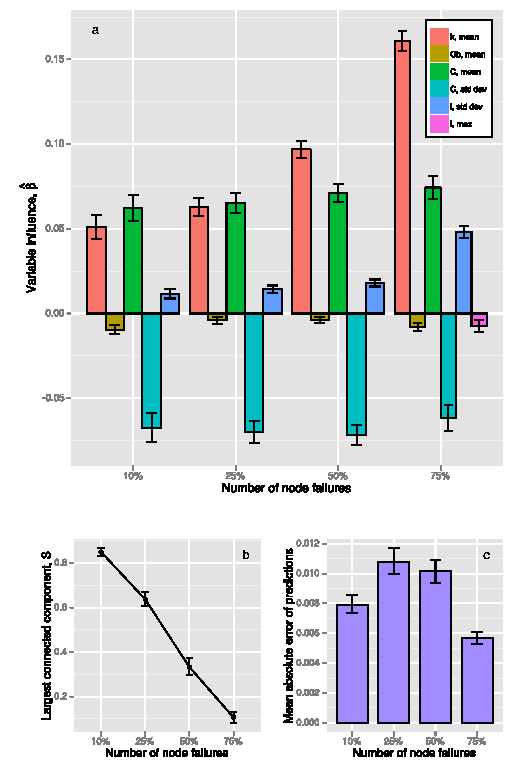
\includegraphics[height=0.95\textheight]{networkModel.pdf}
\caption[Beta regression models of network robustness to random failures]{\label{fig:ch2:betaregNR}Beta regression models of network robustness to random failures as a function of initial network topology.}
\end{center}
\end{figure}

%--------------------------------------------

The mean of the clustering coefficient, $C$, a measure of how locally connected nodes are, is the most important topological characteristic in determining $S$ when small fractions of nodes are removed. For a network of a given degree distribution, higher local connectivity ( \emph{e.g.}, clustering) implies that a more locally redundant set of edges exists. When one node is removed, this locally redundant set of edges decreases the chance that nodes will become disconnected from the network, increasing $S$. My results confirm this. Furthermore, my results show that the influence of $C$ on $S$ remains relatively constant from 10\% of nodes removed through 75\% of nodes removed, though it becomes less influential than nodal degree, $k$, at 50\% and 75\% of nodes removed. Maintaining high local clustering is thus important across a range of magnitudes of impacts to networks, with increased clustering effectively offering local redundancy.

My model shows that the mean of $k$ is nearly as important as $C$ at low levels of node removal but quickly becomes the most influential topological characteristic. An increase in the mean nodal degree of a network implies an increase in the total number of edges between nodes in the network. Thus, the random removal of a node in a network with high mean degree is less likely to disconnect the network than the random removal of that node in a network with lower mean degree; this is confirmed by my results.

In my regression model, $\mu$ is the mean of $S$. With the logit link function, we have:

\begin{equation}
\frac{\partial \frac{S}{1-S}}{\partial x_i} = e^{\beta_i}
\end{equation}
%
This gives a measure of the influence on a given variable, $x_i$, on the ratio of the fraction of connected nodes to the fraction of disconnected nodes after failures. At the 10\% node removal level, increasing the mean of $k$ by 1 unit increases the ratio of fraction connected to fraction disconnected by 1.05 on average, whereas at 75\% node removal, a 1 unit increase in the mean of $k$ increases the ratio of fraction connected to fraction disconnected by 1.17. Note that different results would be expected for targeted node failure events where one might expect higher degree nodes to be targeted for removal first.

The standard deviation of path length also exerts a positive influence on $S$ and its influence increases with number of node failures. However, relative to both the mean of $k$ and $C$, its influence is lower. Higher variability in the path lengths implies greater diversity in the nodes traversed. This additional redundancy in paths between nodes should make it less likely that a given node will be disconnected by node failures, all else being equal in the network. At the same time, the maximum shortest path length is statistically significant only when 75\% of the nodes are removed. Longer shortest path lengths require more nodes to be traversed to maintain connectivity, decreasing the opportunities for path redundancy, again, holding all else fixed. This reinforces the insight that diversity in paths traversed is important because it increases path redundancy.

In contrast to the clustering coefficient mean, increasing its standard deviation negatively influences network robustness, and the absolute value of this influence is approximately equal to that of the (positive) influence of the mean of $C$ across all levels of node removal. To understand this influence it is important to note that the mean of the clustering coefficient is relatively small ($0.29$). As the standard deviation of $C$ increases, it becomes more likely that a node randomly selected for failure would have a low value of $C$. Removing this node would have a larger impact on surrounding nodes because it is not as locally connected as nodes with a higher $C$, leading to an increased chance of additional nodes depending on it but not other nodes becoming disconnected.

Betweenness centrality also exhibits a negative influence on $S$, although its influence is less than that of the other variables. Betweenness centrality of a given node quantifies the relative number of shortest paths that will become longer if that node is removed from the graph. Longer shortest paths are then more susceptible to being severed by other node failures, resulting in decreased network robustness.

In addition to providing a fundamental understanding of the relative influence of different topological characteristics on network robustness, my model can also be used to predict the robustness of real-world power-law networks using simple information about the network's initial topology.  I test my regression models' predictive capabilities on three real-world power-law networks: the Ythan estuary food web \cite{Huxham1996} ($k_{mean} = 8.84$, $Cb_{mean} = 187$, $C_{mean} = 0.217$, $\ell_{mean} = 2.41$) (Figure \ref{fig:ch2:ythan}); the metabolic pathway graph for the bacteria Escherichia coli \cite{Keseler2011} ($k_{mean} = 3.10$, $Cb_{mean} = 806$, $C_{mean} = 0.076$, $\ell_{mean} = 5.43$) (Figure \ref{fig:ch2:eco}); and the terrorist network of 9-11 hijackers and their affiliates \cite{Shaikh2007} ($k_{mean} = 5.00$, $Cb_{mean} = 126$, $C_{mean} = 0.472$, $\ell_{mean} = 3.06$) (Figure \ref{fig:ch2:terr}). Figures \ref{fig:ch2:ythan}-\ref{fig:ch2:terr} present the topology of these networks before and after one set of realizations of random node failures. The color of a node reflects its degree; nodes shown in gray have either been removed or been disconnected from the network as a result of another node failure. As more nodes are removed from the network, its mean topological characteristics (\emph{i.e.}, degree, betweenness centrality, clustering coefficient, and path length) all decrease.

%--------------------------------------------
% FIGURE ------------------------------------

\begin{figure}[!htp]
\begin{center}
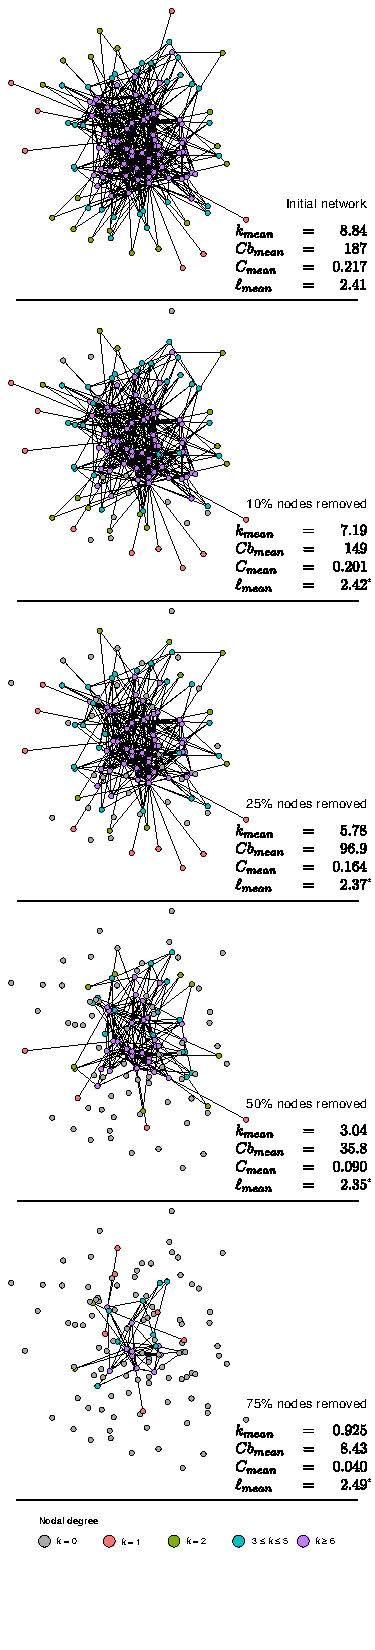
\includegraphics[height=0.95\textheight]{networkYthan.pdf}
\caption[Topology of the Ythan estuary food web.]{\label{fig:ch2:ythan}Topology of the Ythan estuary food web \cite{Huxham1996} before and after one set of realizations of random node failures.}
\end{center}
\end{figure}

%--------------------------------------------

%--------------------------------------------
% FIGURE ------------------------------------

\begin{figure}[!htp]
\begin{center}
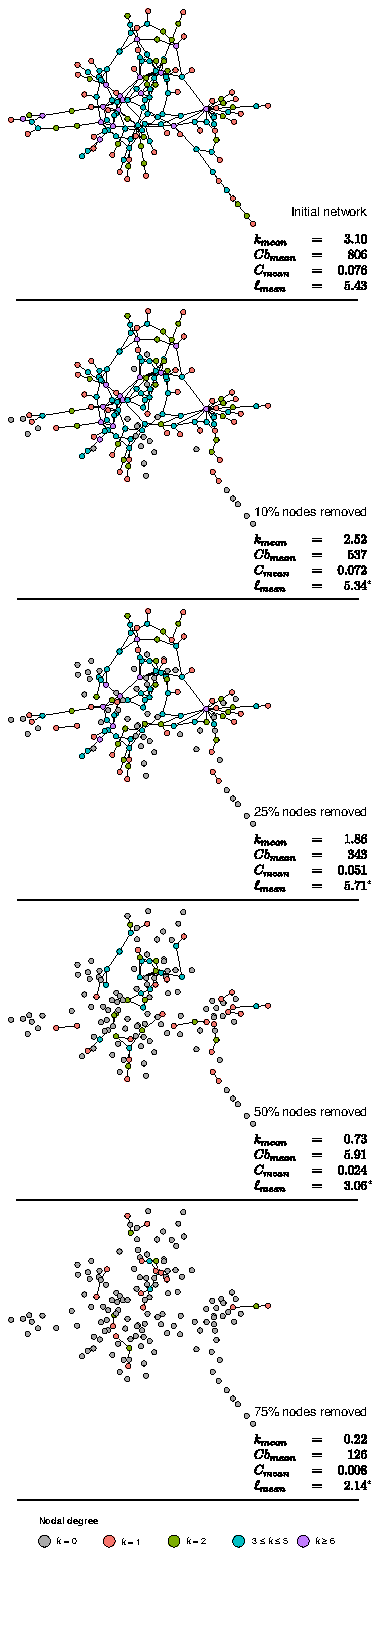
\includegraphics[height=0.95\textheight]{networkEco.pdf}
\caption[Topology of the metabolic pathway graph for the bacteria \emph{Escherichia coli}.]{\label{fig:ch2:eco}Topology of the metabolic pathway graph for the bacteria \emph{Escherichia coli} \cite{Keseler2011} before and after one set of realizations of random node failures.}
\end{center}
\end{figure}

%--------------------------------------------

%--------------------------------------------
% FIGURE ------------------------------------

\begin{figure}[!htp]
\begin{center}
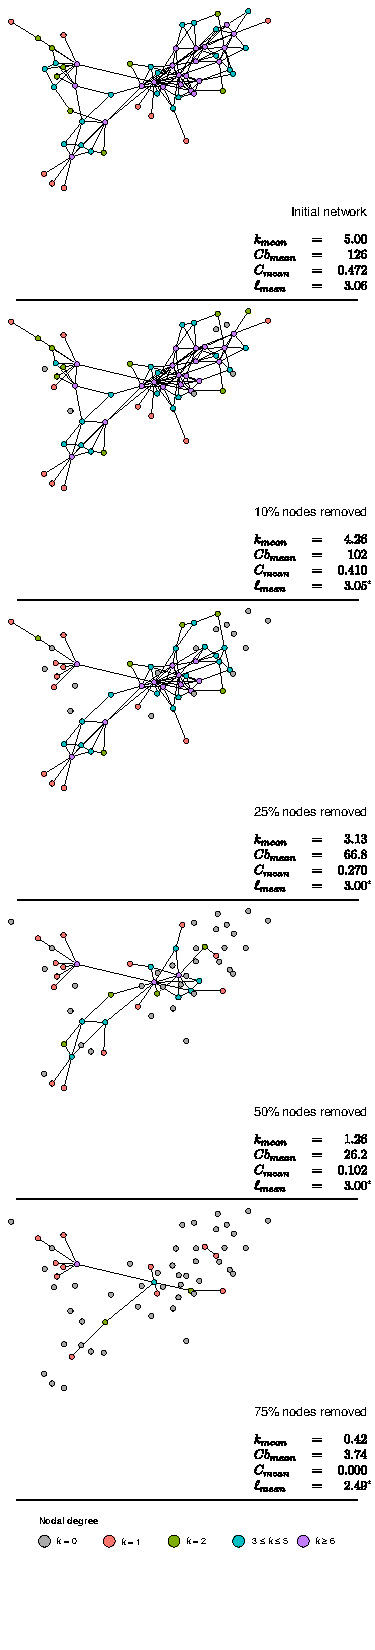
\includegraphics[height=0.95\textheight]{networkTerr.pdf}
\caption[Topology of the terrorist network of 9-11 hijackers.]{\label{fig:ch2:terr}Topology of the terrorist network of 9-11 hijackers \cite{Shaikh2007} before and after one set of realizations of random node failures.}
\end{center}
\end{figure}

%--------------------------------------------

I find that I am able to use my statistical approach to estimate $S$ for these real networks with a high level of accuracy, particularly for small fractions of node removals (\emph{i.e.}, 10\% and 25\%) (Figure \ref{fig:ch2:predict}). In Figure \ref{fig:ch2:predict}, the vertical blue lines show my predictions of network robustness, $S$, for each of the three networks at four levels of node failure. The corresponding histograms give the probability density functions of my simulated $S$ values. The vertical red dashed lines indicate the simulated values of network robustness for each network and failure combination and the vertical pink dashed lines indicated the mean simulated value plus and minus one standard error. The E. coli network was the hardest to predict accurately, with the actual (simulated) $S$ lying outside of the 95\% prediction interval for the two highest levels of node removal. The terrorist network was the easiest to predict accurately, with the 95\% prediction interval containing the true value for all cases.

%--------------------------------------------
% FIGURE ------------------------------------

\begin{figure}[!htp]
\begin{center}
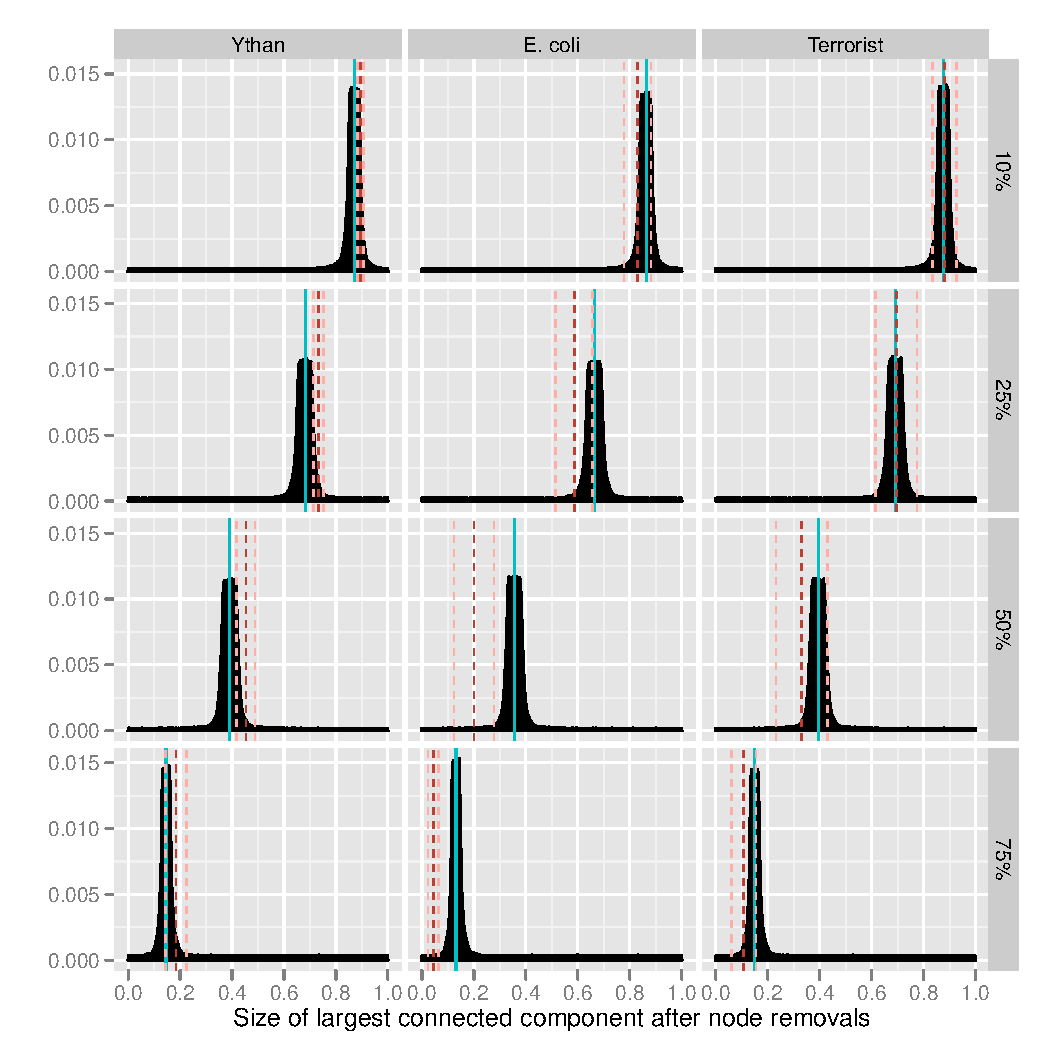
\includegraphics[width=\textwidth]{networkPredict.pdf}
\caption{\label{fig:ch2:predict}Robustness of real-world networks to random node failures: predictions and true values.}
\end{center}
\end{figure}

%--------------------------------------------

I also compare how the regression model and the actual simulation would rank nodes in terms of their importance to the robustness of the network using the example of the terrorist network. To do this, I remove a given node from the network, and determine the value of $S_{10}$ for the modified network simulating random failures in 10\% of the nodes. I repeat this process, removing each node in the original network removed (one at a time). For each of these modified networks, I also use my regression model to predict $S_{10}$. I then rank-order the nodes by $1-S_{10}$ for both the simulation results and the regression predictions. The top three nodes with the simulation-based approach are $33, 21, 5$ in that order. Based on my regression model, the rank-order is $21, 33, 5$ in that order. If nodes are instead ranked based only on nodal degree, the rank-order is $33, 40, 46$. The regression model approximates the rank-ordering of the full simulation model well, at least for the top few most important nodes. A purely degree-based ranking does not match the simulation-based ranking nearly as well. A ranking of the top few nodes in terms of importance to $1-S$ would be of considerable interest to a decision-maker attempting to achieve maximum degradation of network robustness with a minimum number of costly attacks, as would be the case in trying to degrade a terrorist network. My model outperforms a degree-based approach and approximates the full simulation results well for the network of 9/11 terrorists.

%%%%%%%%%%%%%%%%%%%%%%%%%%%%%%%%%%%%%%%%%%%%%%%%%%%%%%%%%%%%%%%%%%%%%%%%%%%

%%%%%%%%%%%%%%%%%%%%%%%%%%%%%%%%%%%%%%%%%%%%%
\subsection{Targeted attacks}
\label{sec:ch2:results:targeted}
%%%%%%%%%%%%%%%%%%%%%%%%%%%%%%%%%%%%%%%%%%%%%

For targeted attacks, four topological characteristics are statistically significant ($p < 0.05$) predictors of network robustness for all four attack schemes at all levels of node failure: mean nodal degree, mean betweenness centrality, mean clustering coefficient, standard deviation of clustering coefficient, and standard deviation of path length.  All of these characteristics are also statistically significant predictors for robustness to random node failures at all levels of node removal.  Incorporating topological characteristics into the statistical model increases its predictions relative to an intercept-only model by a statistically significant amount ($p < 2.2 \times 10^{-16}$). As with random node failures, these results indicate that topological characteristics play a role in determining network robustness and can be used to predict network behavior after incurring targeted attacks.

%--------------------------------------------
\subsubsection{Degree-based attacks}
\label{sec:ch2:results:targeted:degree}
%--------------------------------------------

The direction and magnitude of influence of initial topological characteristics on network robustness are very similar for both types of degree-based attacks. Across all levels of node removal, mean clustering coefficient and standard deviation of path length exert a positive influence on $S$, while mean betweenness and standard deviation of clustering coefficient all negatively influence $S$.  Figures \ref{fig:ch2:betaregNDi} and \ref{fig:ch2:betaregNDr} show the influence of these initial topological characteristics on network robustness to degree-based targeted attacks.  Figures \ref{fig:ch2:meanSNDi} and \ref{fig:ch2:meanSNDr} show that for both types of degree-based attacks, as the number of node failures increases, the relative size of the largest connected component, $S$, decreases.  Results of holdout validation are shown in figures \ref{fig:ch2:maeNDi} and \ref{fig:ch2:maeNDr}, with the purple bars giving the mean absolute errors of the models' predictions and the error bars giving the 95\% confidence intervals for the prediction errors.

%--------------------------------------------
% FIGURE ------------------------------------

\begin{figure}[!htp]
\begin{center}
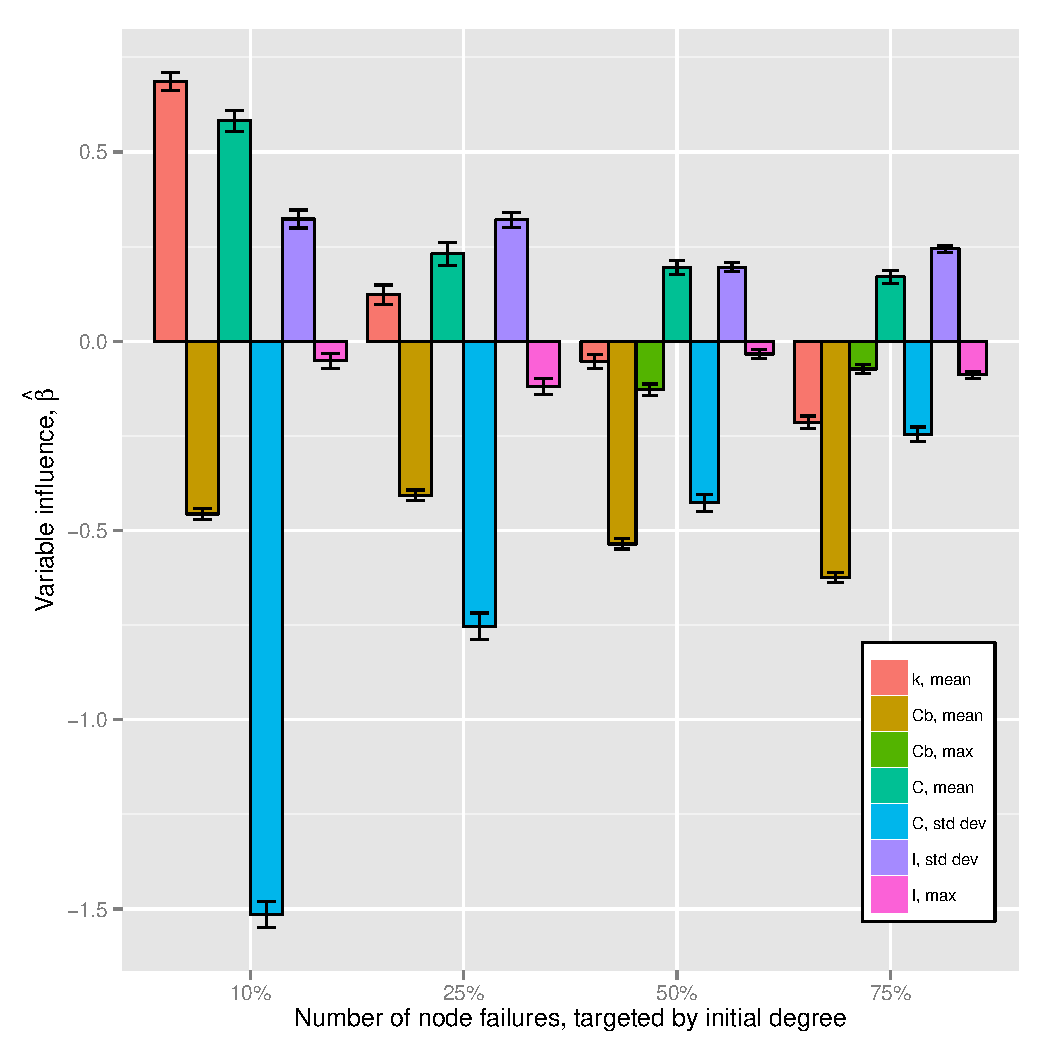
\includegraphics[width=\textwidth]{betareg_NDi_V11.pdf}
\caption{\label{fig:ch2:betaregNDi}Beta regression models of network robustness to initial degree-based attacks as a function of initial network topology.}
\end{center}
\end{figure}

%--------------------------------------------

%--------------------------------------------
% FIGURE ------------------------------------

\begin{figure}[!htp]
\begin{center}
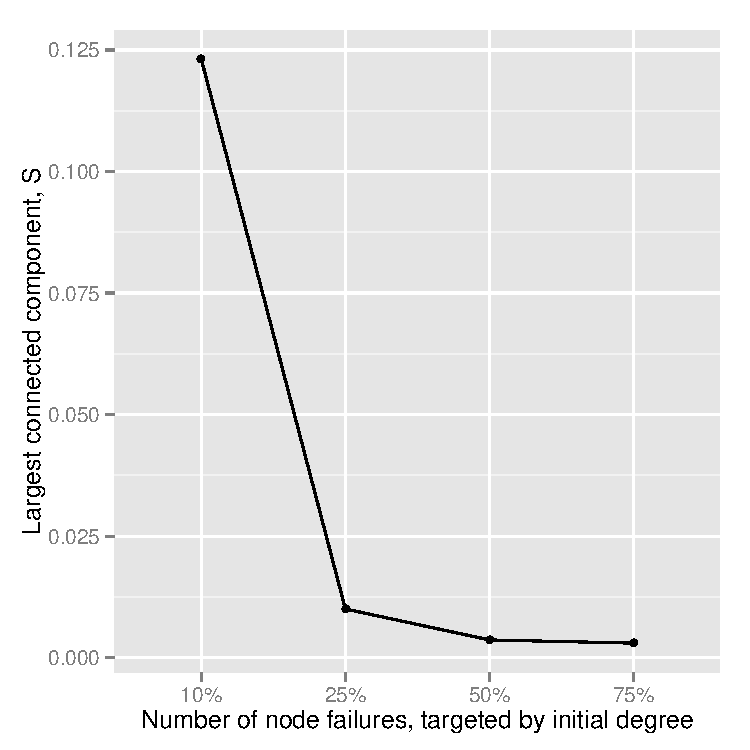
\includegraphics[height=0.4\textheight]{meanS_NDi_V11_v2.pdf}
\caption{\label{fig:ch2:meanSNDi}Relative size of largest connected component, $S$, after initial degree-based attacks.}
\end{center}
\end{figure}

%--------------------------------------------

%--------------------------------------------
% FIGURE ------------------------------------

\begin{figure}[!htp]
\begin{center}
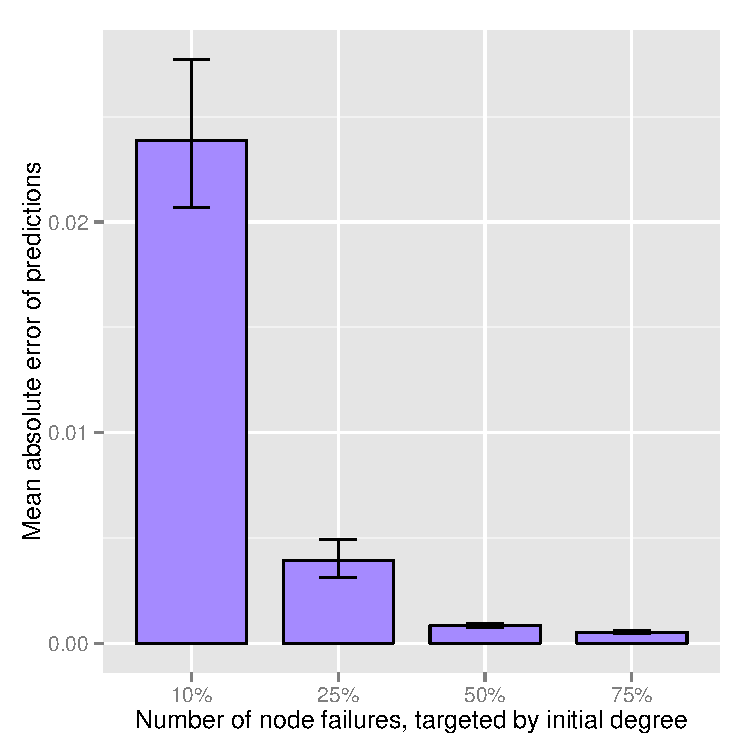
\includegraphics[height=0.4\textheight]{MAE_NDi_V11_v2.pdf}
\caption{\label{fig:ch2:maeNDi}MAEs for holdout validation for initial degree-based attacks.}
\end{center}
\end{figure}

%--------------------------------------------

%--------------------------------------------
% FIGURE ------------------------------------

\begin{figure}[!htp]
\begin{center}
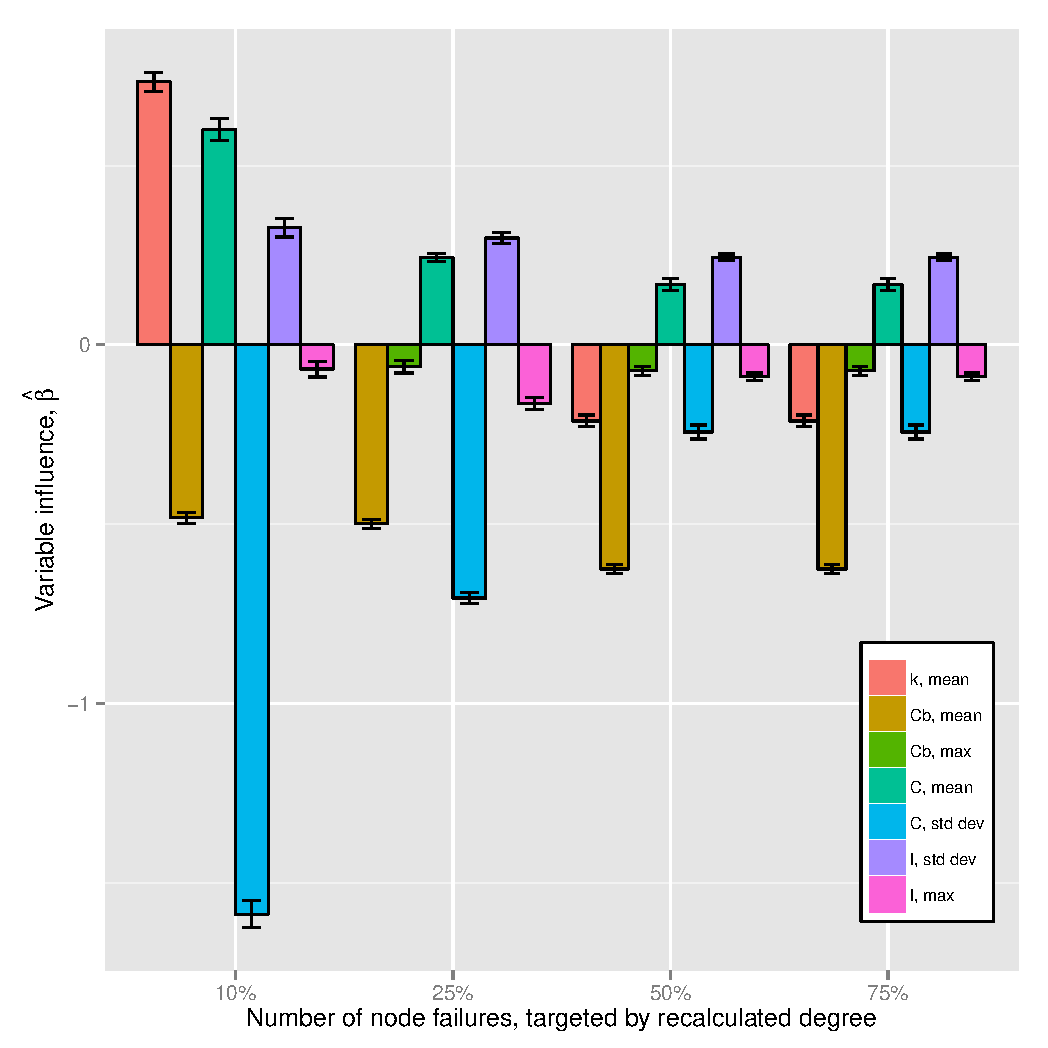
\includegraphics[width=\textwidth]{betareg_NDr_V11.pdf}
\caption{\label{fig:ch2:betaregNDr}Beta regression models of network robustness to recalculated degree-based attacks as a function of initial network topology.}
\end{center}
\end{figure}

%--------------------------------------------

%--------------------------------------------
% FIGURE ------------------------------------

\begin{figure}[!htp]
\begin{center}
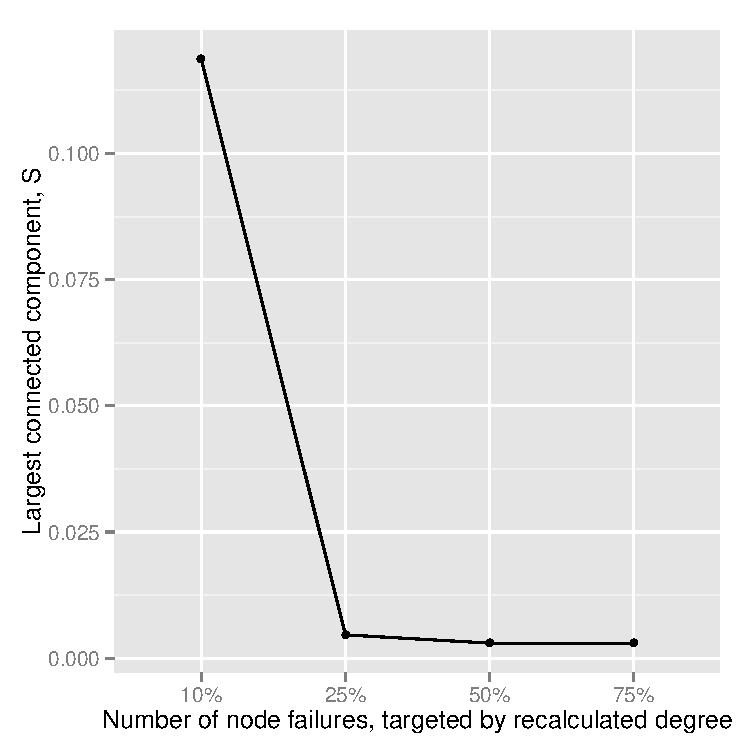
\includegraphics[height=0.4\textheight]{meanS_NDr_V11_v2.pdf}
\caption{\label{fig:ch2:meanSNDr}Relative size of largest connected component, $S$, after recalculated degree-based attacks.}
\end{center}
\end{figure}

%--------------------------------------------

%--------------------------------------------
% FIGURE ------------------------------------

\begin{figure}[!htp]
\begin{center}
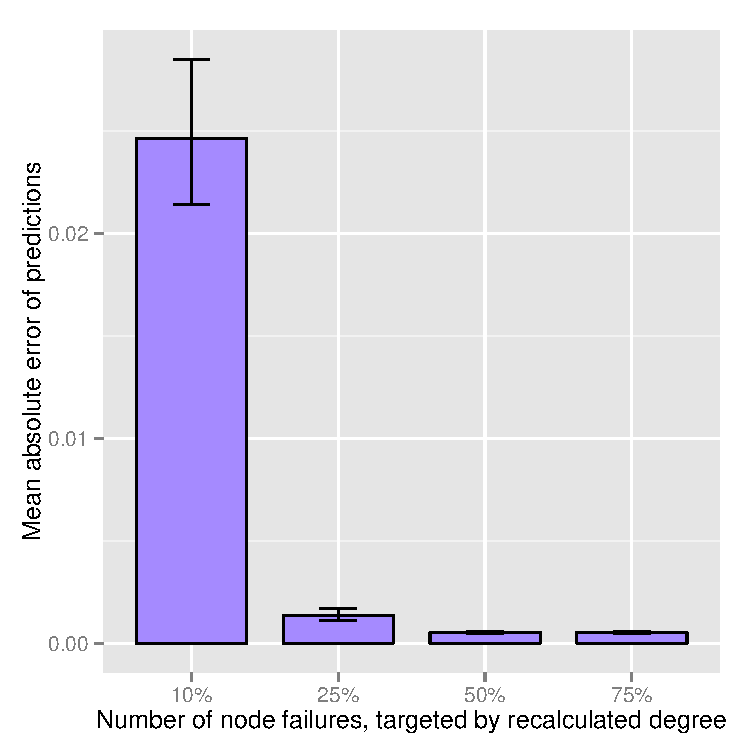
\includegraphics[height=0.4\textheight]{MAE_NDr_V11_v2.pdf}
\caption{\label{fig:ch2:maeNDr}MAEs for holdout validation for recalculated degree-based attacks.}
\end{center}
\end{figure}

%--------------------------------------------

For smaller numbers of nodes removed (\emph{i.e.}, 10\% and 25\%), the standard deviation of clustering coefficient, $C_{std dev}$, is the most important topological characteristic for both types of degree-based attacks, with higher values of $C_{std dev}$ decreasing network robustness.  However, the influence of $C_{std dev}$ decreases significantly as the number of node failures increases, so it is no longer the most important characteristic when larger numbers of nodes are removed. The negative direction of influence of $C_{std dev}$ for degree-based attacks is consistent with the negative direction of influence for random failures. Higher values of $C_{std dev}$ indicate that the network has a greater spread of clustering coefficients, \emph{e.g.}, more nodes with high clustering coefficient and more nodes with low clustering coefficient.  In such a network, the removal of a node with low clustering coefficient is more likely than in a network with smaller $C_{std dev}$. Removing a node with low clustering coefficient will have a larger impact on the network connectivity than a node with higher clustering coefficient, hence the negative influence of $C_{std dev}$ on robustness.

Mean betweenness, $Cb_{mean}$, also exerts a negative influence on network robustness for both types of degree-based attacks.  In contrast to the results from random failures where it had a relatively small negative influence on robustness, $Cb_{mean}$ is the most important topological characteristic for high levels of node removal. One reason that its influence is higher here is that there is likely a correlation between nodal degree and betweenness. Because nodes here are targeted by highest degree, it is likely that nodes with high betweenness are also being targeted. The result of removing nodes with high betweenness is that shortest paths become longer, and thus the network is more susceptible to being severed by further node failures.  Thus $Cb_{mean}$ has a relatively large influence on network robustness to degree-based attacks.  Maximum betweenness, $Cb_{max}$ also has a small influence on robustness for higher levels of node removal (50\% and 75\% for initial degree-based attacks and 25\%, 50\%, and 75\% for recalculated degree-based attacks).

Mean degree, $k_{mean}$, is the only variable whose influence changes direction as the number of node failures increases.  For small numbers of node failures (10\% and 25\% for initial degree-based attacks and 10\% for recalculated degree-based attacks), $k_{mean}$ exerts a positive influence on $S$.  As mentioned in Section \ref{sec:ch2:results:random}, we would expect that increasing the mean of $k$ would have a greater influence on $S$ with targeted attacks than with random attacks.  This is the case for both types of degree-based attacks when 10\% of nodes are removed, with an increase in the mean of $k$ of 1 unit leading to an increase in fraction of nodes connected to nodes disconnected of 1.99 and 2.08 for initial and recalculated degree-based attacks, respectively. However, for higher numbers of node failures (50\% and 75\%), $k_{mean}$ has a negative influence on $S$. With a relatively small number of failures, higher mean degree can be expected to increase robustness to degree-based failures, because even though the initial failed nodes will be the highest degree nodes, there will still be remaining nodes of high degree, reducing the likelihood that an additional failure will disconnect the network. However, as more nodes of high degree fail, the likelihood increases that an additional failure will disconnect the network.

As is the case for random failures, mean clustering coefficient, $C_{mean}$, and standard deviation of path length, $\ell_{std dev}$, each have a positive influence on network robustness to degree-based attacks. The influence of $C_{mean}$ decreases with higher numbers of node failures, while $\ell_{std dev}$ remains fairly constant. When a node fails in a network with higher mean clustering coefficient, it is more likely that the nodes previously connected to the failed node are connected to each other, and thus more likely that all of the nodes previously connected to the failed node remain connected to the largest connected component of the network.

%--------------------------------------------
\subsubsection{Betweenness-based attacks}
\label{sec:ch2:results:targeted:betweenness}
%--------------------------------------------

The results for betweenness-based attacks are very similar to those for degree-based attacks. As with degree-based attacks, mean clustering coefficient and standard deviation of path length exert a positive influence on $S$, while mean betweenness and standard deviation of clustering coefficient all negatively influence $S$ across all levels of node removal.  Figures \ref{fig:ch2:betaregNBi} and \ref{fig:ch2:betaregNBr} show the influence of these initial topological characteristics on network robustness to betweenness-based targeted attacks.  Figures \ref{fig:ch2:meanSNBi} and \ref{fig:ch2:meanSNBr} show the relative size of the largest connected component, $S$, for each level of node failure.  Figures \ref{fig:ch2:maeNBi} and \ref{fig:ch2:maeNBr} show results of the holdout validation for betweenness-based attacks.

%--------------------------------------------
% FIGURE ------------------------------------

\begin{figure}[!htp]
\begin{center}
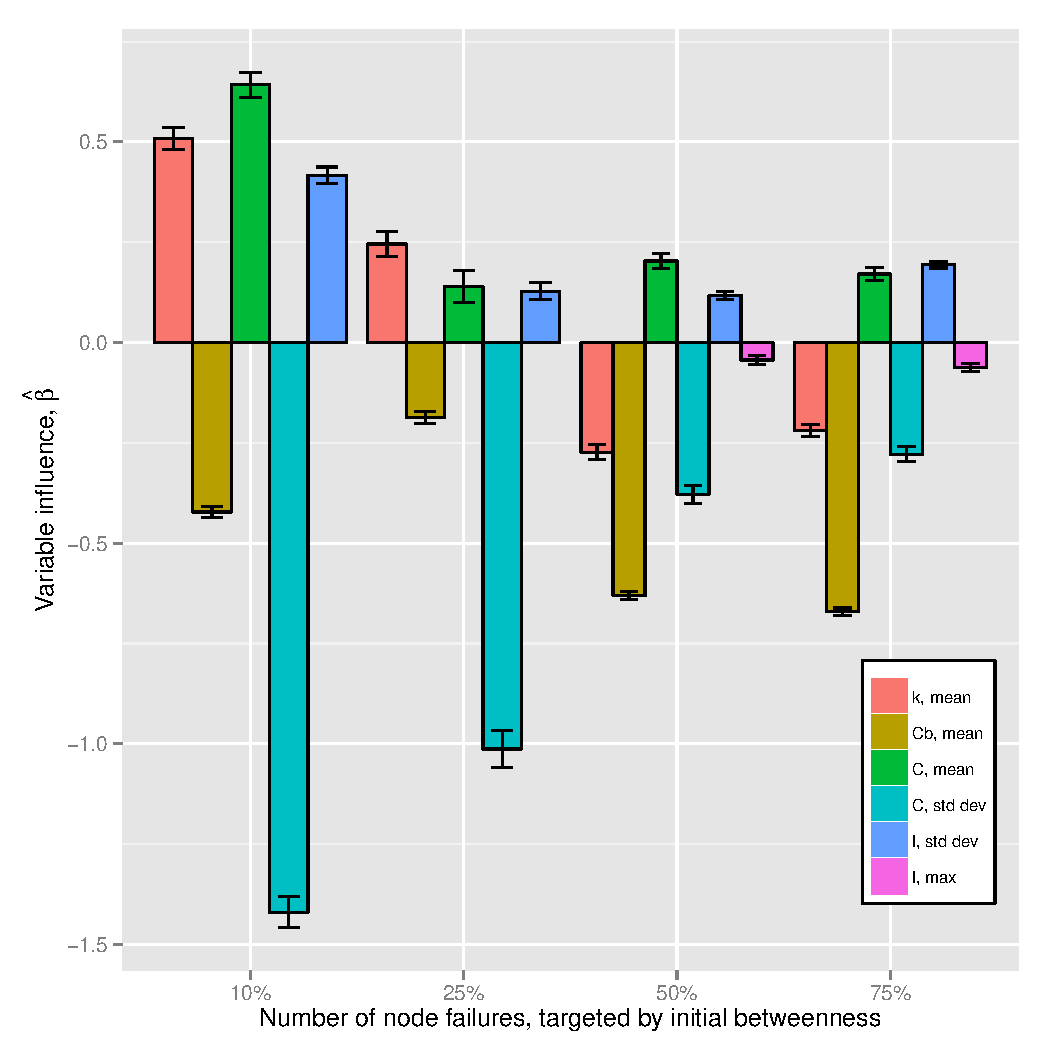
\includegraphics[width=\textwidth]{betareg_NBi_V11.pdf}
\caption{\label{fig:ch2:betaregNBi}Beta regression models of network robustness to initial betweenness-based attacks as a function of initial network topology.}
\end{center}
\end{figure}

%--------------------------------------------

%--------------------------------------------
% FIGURE ------------------------------------

\begin{figure}[!htp]
\begin{center}
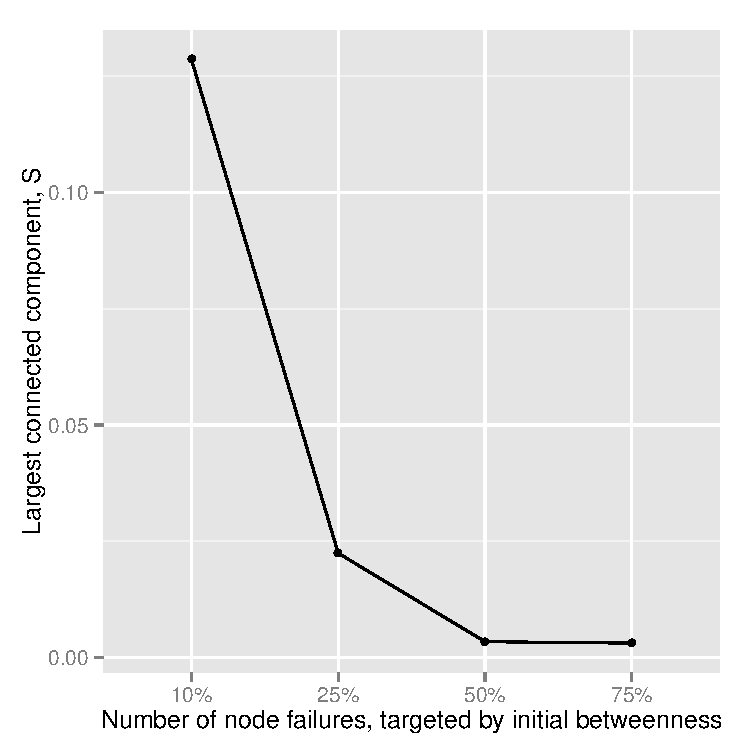
\includegraphics[height=0.4\textheight]{meanS_NBi_V11_v2.pdf}
\caption{\label{fig:ch2:meanSNBi}Relative size of largest connected component, $S$, after initial betweenness-based attacks.}
\end{center}
\end{figure}

%--------------------------------------------

%--------------------------------------------
% FIGURE ------------------------------------

\begin{figure}[!htp]
\begin{center}
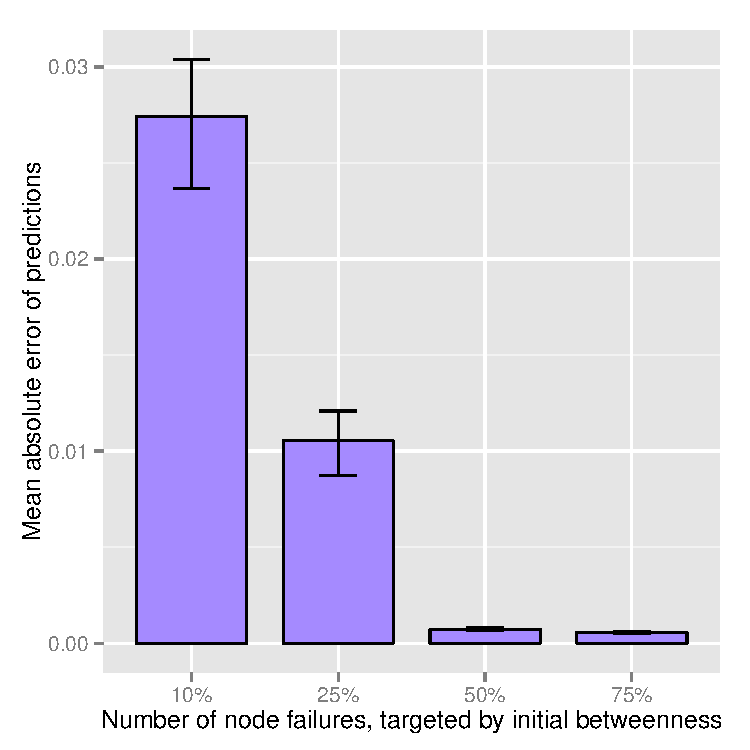
\includegraphics[height=0.4\textheight]{MAE_NBi_V11_v2.pdf}
\caption{\label{fig:ch2:maeNBi}MAEs for holdout validation for initial betweenness-based attacks.}
\end{center}
\end{figure}

%--------------------------------------------

%--------------------------------------------
% FIGURE ------------------------------------

\begin{figure}[!htp]
\begin{center}
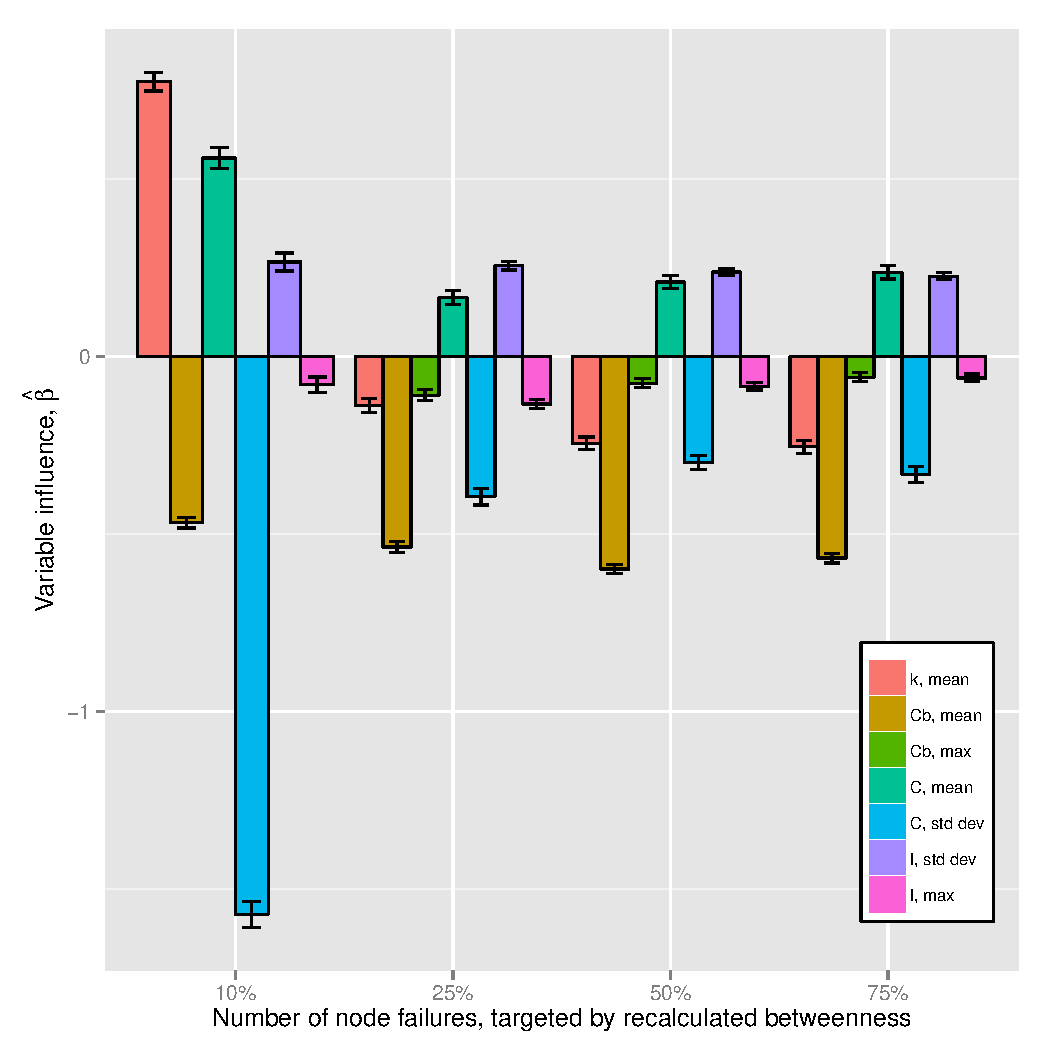
\includegraphics[width=\textwidth]{betareg_NBr_V11.pdf}
\caption{\label{fig:ch2:betaregNBr}Beta regression models of network robustness to recalculated betweenness-based attacks as a function of initial network topology.}
\end{center}
\end{figure}

%--------------------------------------------

%--------------------------------------------
% FIGURE ------------------------------------

\begin{figure}[!htp]
\begin{center}
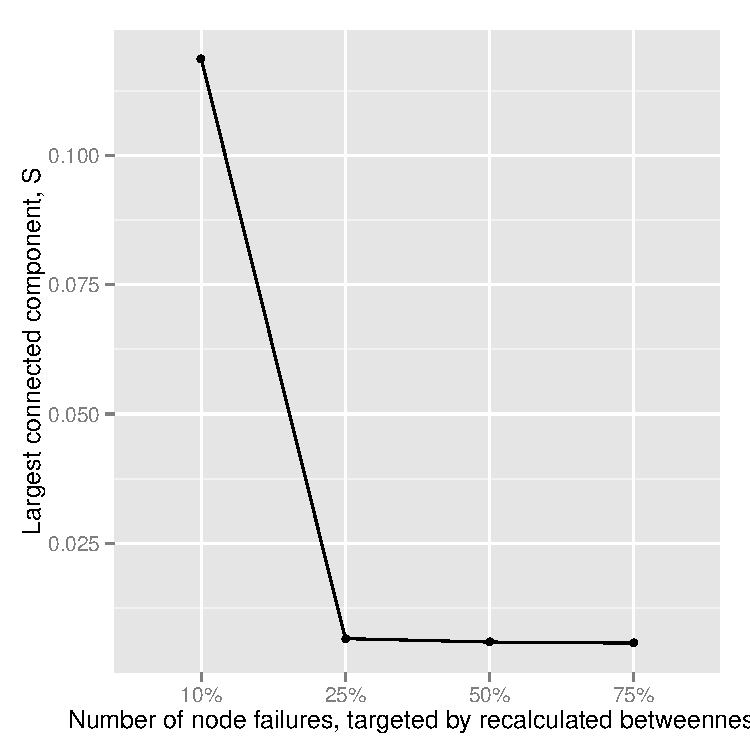
\includegraphics[height=0.4\textheight]{meanS_NBr_V11_v2.pdf}
\caption{\label{fig:ch2:meanSNBr}Relative size of largest connected component, $S$, after recalculated betweenness-based attacks.}
\end{center}
\end{figure}

%--------------------------------------------

%--------------------------------------------
% FIGURE ------------------------------------

\begin{figure}[!htp]
\begin{center}
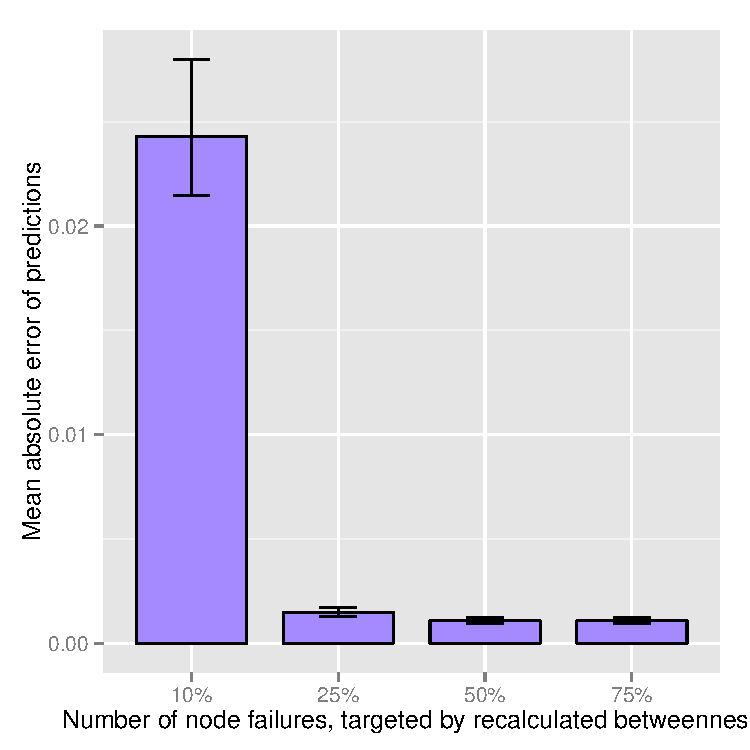
\includegraphics[height=0.4\textheight]{MAE_NBr_V11_v2.pdf}
\caption{\label{fig:ch2:maeNBr}MAEs for holdout validation for recalculated betweenness-based attacks.}
\end{center}
\end{figure}

%--------------------------------------------

As with degree-based attacks, for small numbers of nodes removed, the standard deviation of clustering coefficient, $C_{std dev}$, is the most important topological characteristic for both types of betweenness-based attacks, with higher values of $C_{std dev}$ decreasing network robustness. Again, the influence of $C_{std dev}$ decreases significantly as the number of node failures increases, so it is no longer the most important characteristic when larger numbers of nodes are removed.

Mean betweenness, $Cb_{mean}$, also exerts a negative influence on network robustness for both types of betweenness-based attacks, and is again the most important topological characteristic for high levels of node removal. This finding is expected given that nodes are targeted in order of highest betweenness.  Networks with higher $Cb_{mean}$ will have nodes with higher betweenness attacked, resulting in a higher number of shortest paths removed from the network and decreasing its robustness to additional failures. Maximum betweenness, $Cb_{max}$, also has a small influence on robustness for higher levels (25\%, 50\%, and 75\%) of recalculated degree-based attacks.

The influence of mean degree, $k_{mean}$, changes direction as the number of node failures increases as it did with degree-based attacks. The influence of mean clustering coefficient, $C_{mean}$, and standard deviation of path length, $\ell_{std dev}$, exert a positive influence on $S$ for betweenness-based attacks as was the case with degree-based attacks.

The extreme similarities between the influence of initial topological characteristics for all four types of targeted attacks could have significant real-world implications. Optimal methods for hardening a given network to targeted attacks would be similar for multiple attack strategies, thus potentially simplifying decision-making even when the attacker's specific strategy is not known.  However, the results here also demonstrate that the influence of topological characteristics on network robustness are \emph{not} the same for random failures and targeted attacks.  For example, increasing the mean degree of a network (while keeping other topological characteristics the same) will increase a network's robustness to random failures, but will actually decrease its robustness to large-scale targeted attacks.  Or, increasing the mean betweenness of a network will result in a significant improvement to robustness for targeted attacks, but will have little influence on robustness to random failures.  Therefore, decision-making for improving network reliability must also consider the types of failures that are likely to occur.

%%%%%%%%%%%%%%%%%%%%%%%%%%%%%%%%%%%%%%%%%%%%%%%%%%%%%%%%%%%%%%%%%%%%%%%%%%%%%%%%%%%%%%%%%%%%%%%%

%%%%%%%%%%%%%%%%%%%%%%%%%%%%%%%%%%%%%%%%%%%%%
\section{Conclusions}
\label{sec:ch2:conclusions}
%%%%%%%%%%%%%%%%%%%%%%%%%%%%%%%%%%%%%%%%%%%%%

In summary, I demonstrate that there is a statistically significant relationship between the initial topological properties of my scale-free networks and their corresponding robustness to both random and targeted failures. My statistical models are generalizable to large-scale, realistic networks and provide strong insights into the effects of topology on robustness. For random failures, I find that although the relative influence of different topological measures varies depending on the level of network disturbance ( \emph{e.g.}, number of nodes removed), the direction of the influence of a given characteristic is always the same.  Specifically, higher nodal degree and clustering coefficient, lower betweenness centrality, and lower variability in path length and clustering coefficient imply greater network robustness.  This improved understanding of the impact of network topology on robustness has many applications and benefits in the context of operations research.  Because my models allow for rapidly and accurately estimating network robustness, they can be used to prioritize improvement efforts among multiple existing networks and to allocate resources to those networks. Additionally, such robustness estimates can be incorporated into the optimization of single networks, both for the design of new networks and for improving (or degrading) existing networks.  I show that using my robustness estimates to identify optimal attack strategies on a terrorist network provides a closer match to the true optimal strategy than basing the attack strategy on nodal degree. Finally, the relative simplicity of my models, both in required data and in computational complexity, makes them a highly practical and efficient tool for aiding real-world decision-making.

%%%%%%%%%%%%%%%%%%%%%%%%%%%%%%%%%%%%%%%%%%%%%%%%%%%%%%%%%%%%%%%%%%%%%%%%%%%%%%%%%%%%%%%%%%%%%%%%%%%%%%%%%%%%%%%%%%%%%%%%
